\documentclass[10pt, a4paper, oneside, fontset=none]{ctexart}
%调用宏包
\usepackage{amsmath, amsthm, amssymb, graphicx, wrapfig, mathrsfs, upgreek}
\usepackage[bookmarks=true, colorlinks, citecolor=blue, linkcolor=black]{hyperref}
\usepackage{color, framed, geometry, tcolorbox, multirow, booktabs}
\tcbuselibrary{breakable}%box跨页
\tcbuselibrary{skins}%box跨页不留边
%\usepackage{CJKpunct}
\usepackage{marginnote}
\usepackage{makecell, booktabs, longtable}
\usepackage[font=sf, labelfont+=bf]{caption}
\usepackage[font={small, sf}]{subfig}
\usepackage{multicol}
\usepackage{arydshln, nicematrix}%矩阵
\usepackage{extarrows}
\usepackage[american, cuteinductors, ]{circuitikz}
\usepackage{xpatch}
\usepackage{rotating}%旋转
\usepackage{physics}
\usepackage{siunitx}
\usepackage{enumitem}
\usepackage{listings}
\usepackage{dashrule}
\usepackage[text=\includegraphics{C:/Users/16870/.vscode/LaTeX_Application/tex/THUEE23-23Autumn/图标简稿.png},angle=0]{draftwatermark}%水印
%\usepackage{tikz}
%基本字体设置
\usepackage[math-style=ISO, bold-style=ISO]{unicode-math}
\setmainfont{KpRoman}
%\setmainfont{EB Garamond}
%\setmathfont{Garamond-Math.otf}[StylisticSet={7,9}]
\setmonofont{Iosevka}
\setmathfont{KpMath-Regular.otf}%NewCMMath-Regular
%\setmathfont[range=bb]{TeXGyrePagellaMath-Regular}
%\setmathsfont(Digits,Latin){Garamond MT Pro}
\setmathfont[range={\int}]{NewCMMath-Regular}
\setCJKmainfont{FZXSSK.TTF}[BoldFont={SourceHanSerifCN-Bold.otf}, ItalicFont={FZXKTK.TTF}, BoldItalicFont={汉仪颜楷W.ttf}]
\setCJKsansfont{汉仪文黑-45W.ttf}[BoldFont={汉仪文黑-75W.ttf}, ItalicFont={FZYanZQKSJF.TTF}]
\setCJKmonofont{LXGWNeoXiHei.ttf}
%附加字体设置
\newCJKfontfamily{\kaico}{可口可乐在乎体 楷体Coca-ColaCareFontKaiTi.TTF}
\newCJKfontfamily{\kai}{FZXKTK.TTF}[BoldFont={汉仪颜楷W.ttf}, ItalicFont={方正清刻本悦宋 简繁.TTF}, BoldItalicFont={FZYanZQKSJF.TTF}]
\newCJKfontfamily{\yan}{方正清刻本悦宋 简繁.TTF}[ItalicFont={FZYanZQKSJF.TTF}]
\newCJKfontfamily{\xiu}{方正宋刻本秀楷_GBK.TTF}[ItalicFont={方正宋刻本秀楷_GBK.TTF}, BoldFont={FZYanZQKSJF.TTF}]
\newCJKfontfamily{\run}{汉仪润圆-45W.ttf}[BoldFont={汉仪润圆-75W.ttf}, ItalicFont={汉仪润圆-45W.ttf}]
\newCJKfontfamily{\wen}{汉仪文黑-45W.ttf}[BoldFont={汉仪文黑-75W.ttf}, ItalicFont={hk4e_zh-cn.ttf}]
%文档格式
\geometry{left=2.24cm, right=2.24cm, top=3.18cm, bottom=3.18cm}
\linespread{1.4}
\numberwithin{equation}{section}
\setcounter{tocdepth}{3}
\setcounter{secnumdepth}{4}
\renewcommand{\theparagraph}{\hskip2em\Alph{paragraph})}
\newcommand{\Section}[1]{ \refstepcounter{section} \section*{*\thesection\texorpdfstring{\quad}{} #1} \addcontentsline{toc}{section}{\makebox[0pt][r]{*}\thesection\texorpdfstring{\quad}{} #1} }
\newcommand{\Subsection}[1]{ \refstepcounter{subsection} \subsection*{*\thesubsection\texorpdfstring{\quad}{} #1} \addcontentsline{toc}{subsection}{\makebox[0pt][r]{*}\thesubsection\texorpdfstring{\quad}{} #1} }
\newcommand{\Subsubsection}[1]{ \refstepcounter{subsubsection} \subsubsection*{*\thesubsubsection\texorpdfstring{\quad}{} #1} \addcontentsline{toc}{subsubsection}{\makebox[0pt][r]{*}\thesubsubsection\texorpdfstring{\quad}{} #1} }
\setlist[itemize]{leftmargin=3em, labelsep=0.25em, itemindent=0em, itemsep=0pt, parsep=0pt, topsep=3pt, partopsep=0pt}
\setlist[description]{align=left, leftmargin=2em, itemindent=-1em, labelsep=1em, parsep=0pt, topsep=3pt, partopsep=0pt}
\setlength{\marginparwidth}{8em}
\setlength{\lineskip}{5pt}
\setlength{\lineskiplimit}{5pt}

\setlength{\abovecaptionskip}{0.3em}
\setlength{\belowcaptionskip}{0em}
\captionsetup[subfigure]{captionskip=0.5em, nearskip=0em}
\captionsetup[table]{justification=raggedright,singlelinecheck=false}
\renewcommand{\thefigure}{\thesection.\arabic{figure}}
\renewcommand{\thetable}{\thesection.\arabic{table}}

\tikzset{every node/.style={scale=0.8}}
\ctikzset{monopoles/vcc/arrow={Stealth[width=4pt, length=6pt]}}
\ctikzset{monopoles/vee/arrow={Stealth[width=4pt, length=6pt]}}
\ctikzset{bipoles/length=1cm} %电路图大小标的
\ctikzset{resistors/thickness=2.5}
\ctikzset{voltage=raised}
\ctikzset{bipoles/cuteswitch/thickness=0.4}
\tikzset{ %元件着色
    R/.append style={color=balib},
    C/.append style={color=balib},
    L/.append style={color=balib},
    Do/.append style={color=balib},
    zDo/.append style={color=balib},
    leDo/.append style={color=balib},
    pDo/.append style={color=balib},
    battery1/.append style={color=meihong!75!black},
    battery2/.append style={color=meihong!75!black},
    battery/.append style={color=meihong!75!black},
    cI/.append style={color=meihong!75!black},
    I/.append style={color=meihong!75!black},
    cV/.append style={color=meihong!75!black},
    V/.append style={color=meihong!75!black},
}
\tikzset{bcirc/.style={circ, color=black}}
\tikzset{wcirc/.style={ocirc, color=black, fill=white}}
\ctikzset{
	*-*/.style = {bipole nodes={bcirc}{bcirc}},
	-*/.style = {bipole nodes={none}{bcirc}},
	*-/.style = {bipole nodes={bcirc}{none}},
	o-o/.style = {bipole nodes={wcirc}{wcirc}},
	-o/.style = {bipole nodes={none}{wcirc}},
	o-/.style = {bipole nodes={wcirc}{none}},
	o-*/.style = {bipole nodes={wcirc}{bcirc}},
	*-o/.style = {bipole nodes={bcirc}{wcirc}}
}
\newcommand{\bi}[1]{% name
	\node [currarrow, color=black, anchor=center,
	rotate=\ctikzgetdirection{#1-Iarrow}] at (#1-Ipos) {};
}
\newcommand{\bv}[1]{% name
	\draw [color=black] (#1-Vfrom) .. controls (#1-Vcont1)
	and (#1-Vcont2).. (#1-Vto) node [currarrow,
	sloped, anchor=tip, allow upside down,pos=1]{};
}
\renewcommand{\bf}[1]{% name
	\draw [color=black] (#1-Ffrom) -- (#1-Fto) node [currarrow,
	sloped, anchor=tip, allow upside down,pos=1]{};
}
\ctikzset{!vi/.style={no v symbols, no i symbols, no f symbols}}
%\punctstyle{kaiming}
%定理环境
\theoremstyle{plain}
\newtheorem{theorem}{定理}[subsection]
\newtheorem{definition}{定义}[subsection]
\newtheorem{lemma}[theorem]{引理}
\newtheorem{corollary}[theorem]{推论}
\newtheorem{proposition}[theorem]{命题}

\theoremstyle{definition}
\newtheorem{examplein}[theorem]{\run 例题}
\newtheorem{circum}[theorem]{情形}

\newcommand{\exampleparameter}{0}
\newenvironment{example}[1][0]{% 0/1: no space; 2/3: 5pt space
	\renewcommand{\exampleparameter}{#1}
	\ifnum \exampleparameter>1
		\vspace{10pt}
	\fi
	\hrule
	\vspace{3pt}
	\noindent\hdashrule{\linewidth}{0.5pt}{2pt}
	\vspace{-2em}
	\begin{examplein}
}{% 0/2: -0.5pt space; 1/3: 5pt space
	\end{examplein}
	\vspace{-1em}
	\noindent\hdashrule{\linewidth}{0.5pt}{2pt}\vspace{3pt}
	\hrule
	\ifnum 1=\exampleparameter
		\vspace{10pt}
	\else
		\ifnum 3=\exampleparameter
			\vspace{10pt}
		\else
			\vspace{-0.5pt}
		\fi
	\fi
}

\newenvironment{proofs}[1][\small\proofname]{\begin{pf}[breakable, enhanced jigsaw]\begin{proof}[#1]\small\kai
	\abovedisplayskip=2pt
	\belowdisplayskip=2pt
}{\end{proof}\end{pf}}
\newenvironment{solution}[1][解]{\begin{proofs}[\small\textit{\yan #1}]\renewcommand{\qedsymbol}{$\circledS$}}{\end{proofs}}
\renewcommand{\proofname}{\yan{证明}}

\renewenvironment{cases}[1][l]{\left\{\,\begin{NiceArray}{#1}}{\end{NiceArray}\right.}
%颜色命名
\definecolor{meihong}{rgb}{0.85,0.2,0.47}
\definecolor{bali}{rgb}{0.2,0.6,0.78}
\definecolor{qinglv}{rgb}{0,0.35,0.32}
\definecolor{meihongb}{rgb}{0.85,0.2,0.47}
\definecolor{balib}{rgb}{0.15,0.45,0.58}
\definecolor{qinglvb}{rgb}{0,0.35,0.32}
%box环境
\newtcolorbox{pr}[2][]
{colback=black!5!white,colframe=white!75!black,fonttitle=\sffamily\wen\bfseries,title=#2,#1}
\newtcolorbox[use counter=definition,number within=subsection]{defi}[2][]
{colback=bali!5!white,colframe=bali!75!black,fonttitle=\sffamily\wen\bfseries,title=定义~\thetcbcounter. #2,#1}
\newtcolorbox[auto counter,number within=section]{compl}[2][]
{colback=bali!5!white,colframe=bali!65!black,fonttitle=\sffamily\wen\bfseries,label=#2,title=元件~\thetcbcounter. #2,#1, fontupper=\kai, fontlower=\kai}
\newtcolorbox[use counter=theorem,number within=subsection]{theo}[2][]
{%grow to right by=3.2cm,
colback=meihong!5!white,colframe=meihong!75!black,fonttitle=\sffamily\wen\bfseries,fontupper=\run,title=结论~\thetcbcounter. #2,#1}
\newtcolorbox[use counter=definition,number within=subsection]{defil}[2][]
{colback=bali!5!white,colframe=bali!75!black,fonttitle=\sffamily\wen\bfseries,label=#2,title=定义~\thetcbcounter. #2,#1}
\newtcolorbox[use counter=theorem,number within=subsection]{theol}[2][]
{%grow to right by=3.2cm,
colback=meihong!5!white,colframe=meihong!75!black,fonttitle=\sffamily\wen\bfseries,fontupper=\run,label=#2,title=结论~\thetcbcounter. #2,#1}
\newtcolorbox[auto counter,number within=section]{note}[2][]
{colback=qinglv!5!white,colframe=qinglv!75!black,fonttitle=\sffamily\wen\bfseries,title=注~\thetcbcounter. #2,#1}
\newtcbox{\prenote}[1][]
{left=0.25em,right=0.25em,top=0.25em,bottom=0.25em,width=8.5em,toptitle=0.1em,before skip=0pt,after skip=3pt,colback=gray!5!white,colframe=gray!50!black,fonttitle=\linespread{1}\raggedright\small\sf\bfseries,fontupper=\linespread{1}\small\sf,title=#1}
\newtcolorbox{pf}[1][]
{colback=black!5!white,colframe=white!75!black,#1}
\newtcolorbox{eq}[1][]
{standard jigsaw, colback=meihong!5!white, opacityback=0.7, %grow to right by=3.2cm, 
colframe=meihong!85!black,#1, boxrule=0.4pt, leftrule=10pt, arc=0pt, before skip=7pt, after skip=7pt}
%\newcommand{\mybox}[1]{\tikz[baseline=(MeNode.base)]{\node[rounded corners, fill=gray!20](MeNode){#1};}}

\catcode`\,=\active
\def ,{\textup{,}\hskip0.5em }
\newcommand{\hang}[1][1]{\hangafter 1 \hangindent #1em \noindent}
\newcommand{\page}[1]{\hfill P$_\text{#1}$}
\newcommand{\colors}[1]{\color{#1!75!black}}
\newcommand{\paratitle}[1]{\hang \textbf{\wen #1}\hskip1em}
\newcommand{\tboqi}[1]{\textbf{\xiu\color{qinglv!75!black}#1}}
\newcommand{\mboqi}[1]{\symbf{\xiu\color{qinglv!75!black}#1}}
\newcommand{\tboba}[1]{\textbf{\kai\color{bali!75!black}#1}}
\newcommand{\mboba}[1]{\symbf{\kai\color{bali!75!black}#1}}
\newcommand{\tbome}[1]{\textbf{\run\run\color{meihong!75!black}#1}}
\newcommand{\mbome}[1]{\run\symbf{\run\color{meihong!75!black}#1}}
\newcommand{\adjline}{	\lineskiplimit=3pt
	\lineskip=3pt
	\abovedisplayskip=6pt
	\belowdisplayskip=6pt 
	}
\newcommand{\den}[2][]{\begin{defi}{#1}\adjline
	\kai #2\end{defi}}
\newcommand{\din}[2][]{\begin{theo}{#1}\adjline
	\run #2\end{theo}}
\newcommand{\de}[2][]{\begin{defil}{#1}\adjline
	\kai #2\end{defil}}
\newcommand{\di}[2][]{\begin{theol}{#1}\adjline
	\run #2\end{theol}}
\newcommand{\dep}[3][]{\begin{defi}{#1\page{#2}}\adjline
	\kai #3\end{defi}}
\newcommand{\dip}[3][]{\begin{theo}{#1\page{#2}}\adjline
	\run #3\end{theo}}
\newcommand{\zhu}[2][]{\begin{note}{#1}\adjline
	\xiu #2\end{note}}
\newcommand{\bu}[3][]{\begin{compl}{#1}	\paratitle{记号}#2 \tcblower\paratitle{特性}#3\end{compl}}
\newcommand{\trans}[3][2]{\begin{wrapfigure}[#1]{R}{8.7em}
		\vspace{-1.5em}
		\prenote[#2]{\parbox[l]{8em}{\raggedright #3}}
	\end{wrapfigure}}
% \newcommand{\tranS}[3][-1]{\marginnote{
% 		\begin{prenote}{#2}
% 			\raggedright
% 			#3
% 		\end{prenote}
% 	}[#1\baselineskip]}
\newcommand{\cbox}[2][]{
	$\vcenter{\hbox{\begin{circuitikz}[#1]
		#2
	\end{circuitikz}}}$
	}
\newcommand{\shbox}[1]{\cbox{\draw (0,0) to[#1] (1.5,0);}(\texttt{#1})}
%定义算符
\newcommand{\rref}{\symup{rref}}
\newcommand{\C}{\mathbb{C}}
\renewcommand{\i}{\symsf{j}}
\newcommand{\neiji}[4]{\symbf{#1}_{#3}^\symup{T}\symbf{#2}_{#4}}
\def\upint{\mathchoice%
	{\mkern13mu\overline{\vphantom{\intop}\mkern7mu}\mkern-20mu}%
	{\mkern7mu\overline{\vphantom{\intop}\mkern7mu}\mkern-14mu}%
	{\mkern7mu\overline{\vphantom{\intop}\mkern7mu}\mkern-14mu}%
	{\mkern7mu\overline{\vphantom{\intop}\mkern7mu}\mkern-14mu}%
	\int}
\def\lowint{\mkern3mu\underline{\vphantom{\intop}\mkern7mu}\mkern-10mu\int}
\renewcommand{\a}[1]{\left\langle #1 \right\rangle}
\renewcommand{\v}{\vee}
\newcommand{\A}{\wedge}
\renewcommand{\c}[1]{\symbfsfit{#1}}
\newcommand{\V}{\c{V}}
\newcommand{\I}{\c{I}}
\newcommand{\G}{\c{G}}
\newcommand{\Lr}{\Leftrightarrow}
\newcommand{\LLr}[2][]{\xLongleftrightarrow[#1]{#2}}
\newcommand{\rl}{\rightleftarrows}
\newcommand{\dif}{\mathop{}\!\symup{d}}
\newcommand{\Dif}{\mathop{}\!\symup{\Delta}}
\newcommand{\e}{\symup{e}}
\newcommand{\R}{\mathbb{R}}
\newcommand{\bF}{\mathbb{F}}
\newcommand{\dint}{\displaystyle\int}
\newcommand{\dt}[1][]{\dfrac{\dif #1}{\dif t}}
\renewcommand{\ang}[1]{\vcenter{\hbox{\begin{tikzpicture}
	\node (box) at (0,0) {$#1$};
	\draw (box.south west) ++ (-0.05,0.08) coordinate(left)
	(box.south east) ++ (-0.1,0.08) -- (left) -- ++ (0.17,0.45);
\end{tikzpicture}}}\!\!}
\newcommand{\meshcurrent}[2]{\draw[latex-] #1 node{#2} +(0.43,0.25) arc(30:330:0.5);
}
\newcommand{\equ}[1]{\begin{eq}
%	\setmathfont{GFSNeohellenicMath.otf}
	\setmathfont{FiraMath-Regular.otf}\sffamily
	\begin{equation}
		{\color{meihong!85!black} #1}
	\end{equation}\end{eq}
\setmathfont{KpMath-Regular.otf}
\setmathfont[range={\int}]{NewCMMath-Regular}
}
\newcommand{\mrm}[1]{{\symup{#1}}}
\newcommand{\uni}[1]{{\symup{\,#1}}}
%\setmathfont{Garamond-Math.otf}[StylisticSet={7,9}]}
%标题、作者、日期
\title
{
	\textbf{Basic Engineering Circuit Analysis\\电子电路启蒙教程}
}
\author{\zihao{5} T$^\text{T}$T}
\date{\zihao{5} \kai \today}
%----------------------------------------------------------
\begin{document}

\adjline

\maketitle
\begin{multicols}{2}
	\begin{flushleft}
		\tableofcontents
	\end{flushleft}
\end{multicols}

%\newgeometry{left=2.24cm, right=5.14cm, top=3.18cm, bottom=3.18cm}
\newpage
\setcounter{section}{4}
%----------------------------------------------------------
\section{运算放大器与反馈设计}

\subsection{运算放大器}

\ctikzset{amplifiers/fill=bali!25!white}

\bu[运算放大器(operational amplifier)]{
	\cbox{
		\draw (0,0) node[left](IN){$v_p$} to[short, o-] ++(0.2,0) node[op amp, noinv input up, anchor=+](AMP){}
		(AMP.-) to[short, -o] ++(-0.2,0) node[left]{$v_n$}
		(AMP.out) to[short, -o] ++(0.2,0) node[right](OUT){$v_o$}
		(AMP.up) -- ++(0,0.2) node[vcc]{$V_{CC}$} 
		(AMP.down) -- ++(0,-0.2) node[vee]{$V_{EE}$} 
		;
	}(\texttt{op amp, noinv input up})
}{
	在直流电压$V_{CC},V_{EE}$驱动下,输出端点相对接地的电压$v_o=A_v(v_p-v_n)$。
}
我们可以用前面的组件构建运放器的简单模型,如图~\ref{Pic: A simple model for an op-amp}。
\begin{figure}[ht!]
	\begin{center}
		\vspace{-1em}
		\subfloat[Linear区的电路模型]{
			\begin{circuitikz}
				\draw (0,0) to[short, o-, f=$i_p$, !vi, name=ip] ++(1,0) 
					-- ++(1,0)
					to[R, l^=$R_i$, v_=$v_{\symup{in}}$, voltage shift=1] ++(0,-1.5) 
					to[short, -o, f<=$i_n$, !vi, name=in] ++(-1,0) 
					to[open, o-, v=$v_n$] ++(0,-1)
				(0,0) to[open, o-o, v=$v_p$] ++(0,-2.5) 
					to[short, o-*] ++(3,0) node[ground]{} 
					to[short, *-o] ++(2,0)
					to[open, o-o, v<=$v_o$] ++(0,2) 
					to[R, l=$R_o$, o-, label distance=-8pt, f<_=$i_o$, !vi, name=io] ++(-2,0) 
					to[cV, l=$A_vv_{\symup{in}}$] ++(0,-2)
				;
				\bf{in}\bf{ip}\bf{io}
			\end{circuitikz}
		}
		\qquad
		\subfloat[增益曲线]{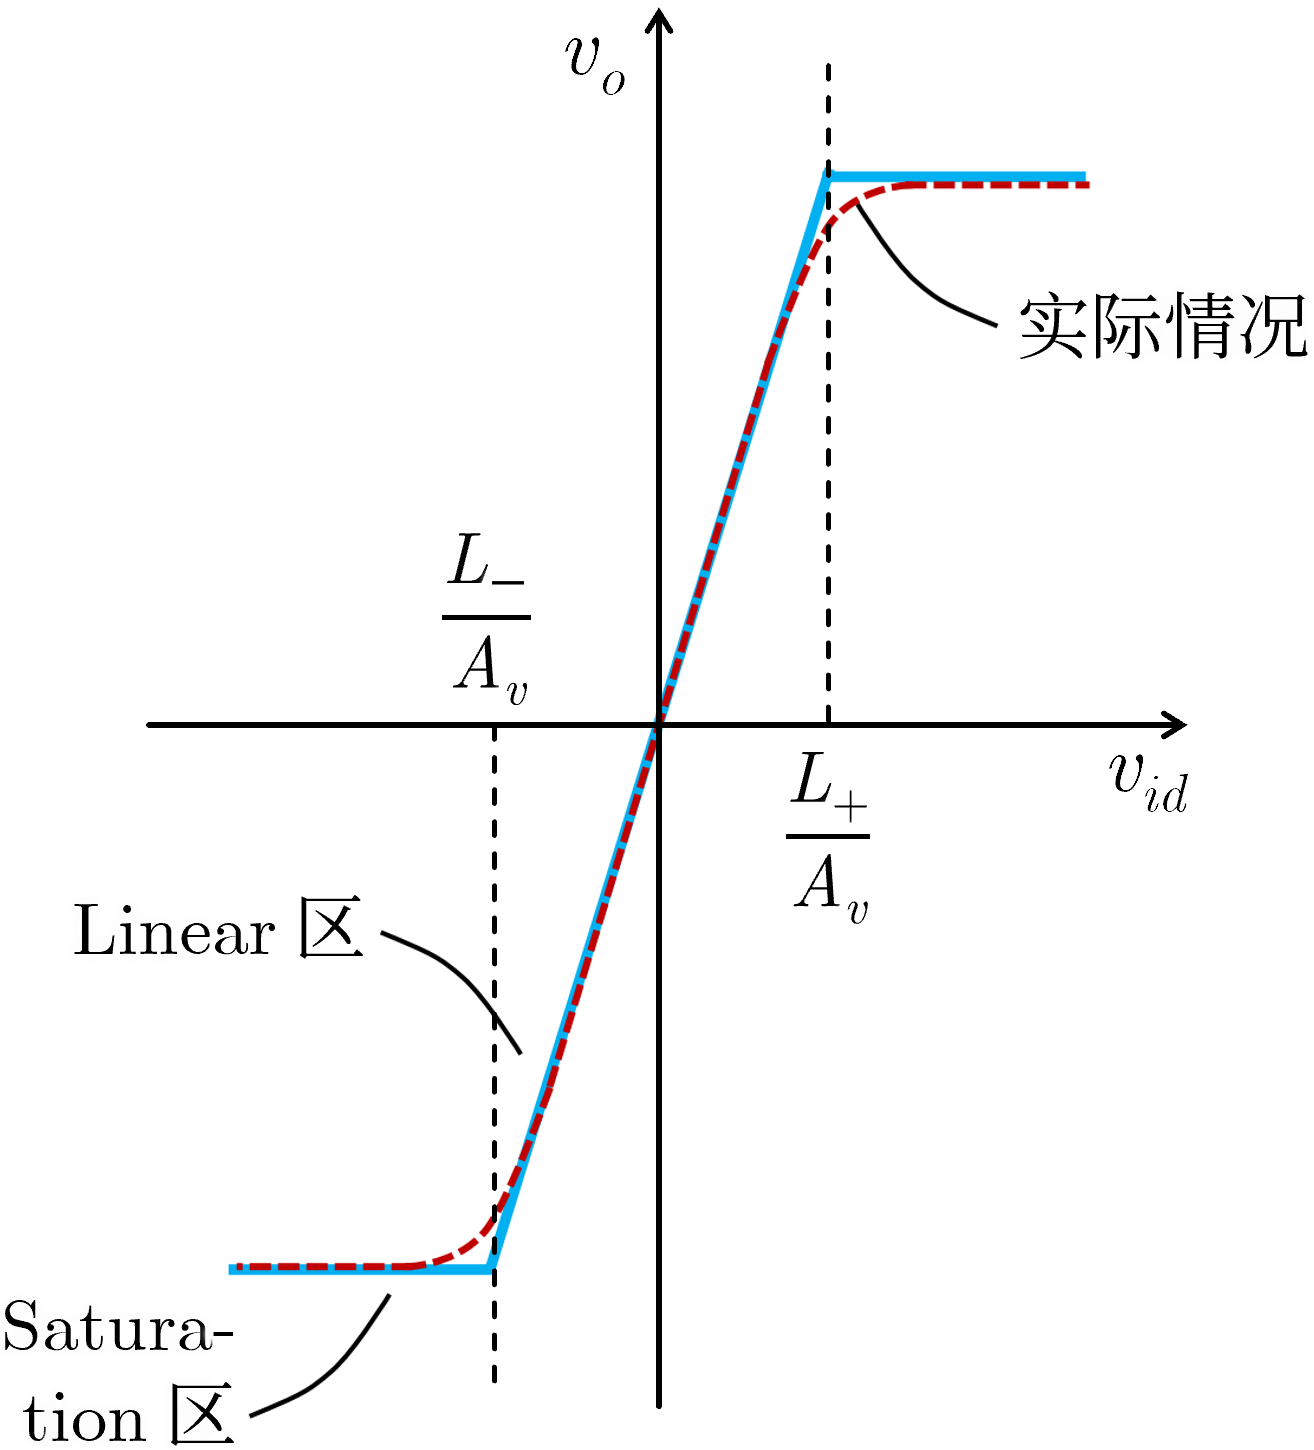
\includegraphics[width=5cm]{opamp vv.png}}
		\caption{运放器的增益特性模型}\label{Pic: A simple model for an op-amp}
		\vspace{-1.5em}
	\end{center}
\end{figure}

\newcommand{\pzcdetector}[2][(0,0)]{%1: position of input; %2: label
	\draw #1 node[plain amp, anchor=in up](#2){};
	\draw (#2.center) ++(-0.25,0) -- ++(0.1,0) 
	(#2.center) ++(-0.25,0) -- ++(-0.1,0) 
	(#2.center) ++(-0.25,0) -- ++(0,0.25) -- ++(0.1,0)
	(#2.center) ++(-0.25,0) -- ++(0,-0.25) -- ++(-0.1,0)
	(#2.in up) coordinate(#2-in)
	(#2.in down) coordinate(#2-ref)
	(#2.out) coordinate(#2-out)
	;
}
\newcommand{\nzcdetector}[2][(0,0)]{%1: position of input; %2: label
	\draw #1 node[plain amp, anchor=in down](#2){};
	\draw (#2.center) ++(-0.25,0) -- ++(0.1,0) 
	(#2.center) ++(-0.25,0) -- ++(-0.1,0) 
	(#2.center) ++(-0.25,0) -- ++(0,0.25) -- ++(-0.1,0)
	(#2.center) ++(-0.25,0) -- ++(0,-0.25) -- ++(0.1,0)
	(#2.in up) coordinate(#2-ref)
	(#2.in down) coordinate(#2-in)
	(#2.out) coordinate(#2-out)
	;
}

\begin{wrapfigure}{r}{4cm}
	\vspace{-2.5em}
	\centering
	\begin{circuitikz}
		\draw (0,0) node[left](G){$v_p$} to[short, o-, i=$i_p$] ++(1.2,0) node[op amp, noinv input up, anchor=+](A){$\infty$}
		(A.- -| G) to[open] ++(0.8,0) node[left](2){$v_n$} to[short, i=$i_n$, o-] (A.-)
		(A.down) node[ground]{}
		(A.out) to[short, -o] ++(0.5,0) node[right]{$v_o$}
		;
	\end{circuitikz}
	\captionof{figure}{理想运算放大器}\label{Pic: Ideal op amp}
	\vspace{-2.5em}
\end{wrapfigure}
实际的运算放大器一般有较大的$A_v$值($10^4 \sim 10^8$)和$R_i$($10^6 \sim 10^{13} \,\mrm{\Omega}$)以及较小的$R_o$($1 \sim 100 \,\mrm{\Omega}$)。因此,可以假设$A_v=\infty,R_i=\infty,R_o=0$,这样的运算放大器称为\tboba{理想运算放大器},如图~\ref{Pic: Ideal op amp}~所示。当理想运放工作在 Linear区 时,有
$$i_p=i_n=0,\qquad v_p=v_n$$
因此,只要$v_p \neq v_n$,理想运放的输出电平就只能为$\pm V_{dd}$。

\trans{过零检测器}{zero-crossing detector}
理想运放的一个直接应用是比较输入端两个信号(通常是输入信号\(v_\mrm{in}\)和参照信号\(v_\mrm{ref}\))的大小,称为\tboba{过零检测器},记为\!\!%
\cbox{
	\pzcdetector{pzcd}
	\draw (pzcd-in) to[short, -o] ++(-0.25,0) node[left]{$v_\mrm{in}$}
	(pzcd-ref) to[short, -o] ++(-0.25,0) node[left]{$v_\mrm{ref}$}
	(pzcd-out) to[short, -o] ++(0.25,0) node[right]{$v_o$}
	;
}\!\!或\!\!%
\cbox{
	\nzcdetector{nzcd}
	\draw (nzcd-in) to[short, -o] ++(-0.25,0) node[left]{$v_\mrm{in}$}
	(nzcd-ref) to[short, -o] ++(-0.25,0) node[left]{$v_\mrm{ref}$}
	(nzcd-out) to[short, -o] ++(0.25,0) node[right]{$v_o$}
	;
}\!\!,前者在\(v_\mrm{in} > v_\mrm{ref}\)时输出高电平,后者在\(v_\mrm{in} < v_\mrm{ref}\)时输出高电平。基于过零检测器可以构建简单的\textbf{模数转换器(ADC)}。

\zhu[模拟信号与数字信号]{
	与实际物理量变化形式类似的电信号称为\tboqi{模拟信号}%\trans[模拟/数字信号]{analog/digital signal}
	。在模拟信号上等时间间距地\textbf{采样}并用有限位数的数字表示采样值的大小,就得到\tboqi{数字信号}。数字信号常以二进制表示,在电信号上表现为只有\tboqi{高电平(1)}和\tboqi{低电平(0)}。%\trans[高/低电平]{high/low voltage level}
	
	要将模拟信号转换为数字信号,需要用到如图~\ref{Pic: ADC}~所示的\tboqi{模数转换器}%\trans[模数转换器]{analog-to-digital converter,\textbf{ADC或A/D}}
	,其在输入端接入模拟电信号,在$N$个输出端输出$N$位二进制数表示的数字信号。
	
	\begin{center}
		\ctikzset{blocks/fill=bali!25!white}
		\begin{circuitikz}
			\filldraw[draw=black, thick, fill=qinglv!25!white] (0,0) rectangle (4,4);
			\node[text centered] at (2,2) {\kai ADC或A/D};
			\draw (0,1) to[short, -o] (-1,1) to[open, o-o, v=$v_\textup{A}$] (-1, 3) to[short, o-] (0,3);
			\draw (4,3) to[short, -o] ++(1,0) node[right]{$d_0$};
			\draw (4,2.5) to[short, -o] ++(1,0) node[right]{$d_1$};
			\draw[dotted, very thick] (4.5,2.35) -- (4.5,1.65);
			\draw (4,1.5) to[short, -o] ++(1,0) node[right]{$d_{N-1}$};
			\draw (4,1) -- ++(0.5,0) node[ground]{};

			\draw (6.5,2) to[adc, o-o] ++(2,0);
		\end{circuitikz}
	\end{center}
	\captionof{figure}{模数转换器}\label{Pic: ADC}
}

\begin{example}
	求电路输出\(\overline{D_2D_1D_0}_{(2)}\)与输入信号\(v_\mrm{in}\)的关系。
	\begin{center}
		\cbox{
			\draw (0,0) node[vcc](Ref){\(v_\mrm{ref}\)}
			(1,0) node[vcc](In){\(v_\mrm{in}\)} 
				-- ++(0,-0.5) -- +(0.5,0) coordinate(In2)
				(In2 -| In) -- ++(0,-1.5) -- +(0.5,0) coordinate(In1)
				(In1 -| In) -- ++(0,-1.5) -- +(0.5,0) coordinate(In0);
			\pzcdetector[(In2)]{D2}\pzcdetector[(In1)]{D1}\pzcdetector[(In0)]{D0}
			\node at (D2-ref -| In) [jump crossing](D2J){};
			\draw (D2-out) to[short, -o] ++(0.5,0) node[right]{\(D_2\)}
			(D2-ref) -- (D2J.east)
			(D2J.west) to[short, -*] (D2-ref -| Ref) node[left]{\(v_2\)};
			\node at (D1-ref -| In) [jump crossing](D1J){};
			\draw (D1-out) to[short, -o] ++(0.5,0) node[right]{\(D_1\)}
			(D1-ref) -- (D1J.east)
			(D1J.west) to[short, -*] (D1-ref -| Ref) node[left]{\(v_1\)};
			\draw (D0-out) to[short, -o] ++(0.5,0) node[right]{\(D_0\)}
			(D0-ref) to[short, -*] (D0-ref -| Ref) node[left]{\(v_0\)};
			\draw (Ref) to[R, l_=\(1.5R\)] (D2-ref -| Ref)
				to[R, l_=\(R\)] (D1-ref -| Ref)
				to[R, l_=\(R\)] (D0-ref -| Ref)
				to[R, l_=\(0.5R\)] ++(0,-1) node[ground]{};
		}
	\end{center}
	\begin{solution}
		由KVL,知\(v_0 = \dfrac{1}{8}v_\mrm{ref},v_1 = \dfrac{3}{8}v_\mrm{ref},v_2 = \dfrac{5}{8}v_\mrm{ref}\),则 
		\begin{equation*}
			\overline{D_2D_1D_0}=\begin{cases}[ll]
				000,& v_\mrm{in} < \dfrac{1}{8}v_\mrm{ref}, \\
				001,& \dfrac{1}{8}v_\mrm{ref} < v_\mrm{in} < \dfrac{3}{8}v_\mrm{ref}, \\[3pt]
				011,& \dfrac{3}{8}v_\mrm{ref} < v_\mrm{in} < \dfrac{5}{8}v_\mrm{ref}, \\
				111,& v_\mrm{in} > \dfrac{5}{8}v_\mrm{ref}
			\end{cases}
			\qedhere
		\end{equation*}
	\end{solution}
\end{example}
\subsection{运算放大器上的反馈回路}

\begin{example}[2]
	已知\textbf{单位增益缓冲器}的电路结构如图~\ref{Pic: Circuit - unity gain buffer}~所示,图~\ref{Pic: Model - unity gain buffer}~是其特性模型。若$A_o \gg 1,R_o \ll R_i$,由此考虑$\dfrac{V_o }{V_S }$的值。
	%\trans[单位增益缓冲器]{unity gain buffer}

	\begin{figure}[ht!]
		\vspace{-1.5em}
		\centering
		\subfloat[电路]{\label{Pic: Circuit - unity gain buffer}
			\begin{circuitikz}
				\draw (0,0) node[ground](G){} to[V, v=$V_S$, invert] ++(0,2) 
				-- ++(1,0) node[op amp, noinv input up, anchor=+](AMP){}
				(AMP.-) -- (G -| AMP.-) coordinate(1) 
				-- (1 -| AMP.out) -- (AMP.out) 
				to[short, -o] ++(1,0) coordinate(3)
				to[open, o-o, v=$V_o$] (G -| 3) to[short, o-] ++(-0.5,0) node[ground]{}
				(AMP.up) -- ++(0,0.2) node[vcc]{$V_{CC}$} 
				(AMP.down) -- ++(0,-0.2) node[vee]{$V_{EE}$} 	
				;
			\end{circuitikz}
		}\qquad
		\subfloat[模型]{\label{Pic: Model - unity gain buffer}
			\begin{circuitikz}
				\draw (0,0) node[ground](G){} to[V, v=$V_S$, invert] ++(0,3) 
				-- ++(1,0) to[R, l=$R_i$, v_=$V_{\symup{in}}$, voltage=raised, voltage shift=-0.7] ++(0,-1.5) 
				-- ++(1,0) -- ++(0,1.5) -- ++(2,0) -- ++(0,-1) coordinate(1) to[short, -o] ++(0.5,0) to[open, o-o, v=$V_o$] ++(0,-2) to[short, o-] ++(-0.5,0) node[ground]{}
				(1) to[R, l=$R_o$, label distance=-8pt] ++(-1.5,0) to[cV, v_=$A_oV_{\symup{in}}$, voltage shift=-0.7] ++(0,-2) node[ground]{}
				;
				\draw[latex-] (1.25,0.25) node{$I$} +(0.43,0.25) arc(30:330:0.5);
			\end{circuitikz}
		}
		\caption{单位增益缓冲器}
		\vspace{-1em}
	\end{figure}
\begin{solution}
	由图易知$V_{\symup{in}}=IR_i$,且有
	\abovedisplayskip=0pt
	\belowdisplayskip=2pt 
	\begin{align*}
		V_S &= IR_i + IR_o + A_oV_{\symup{in}}\\[-3pt]
		V_o &= A_oV_{\symup{in}} +IR_o
	\end{align*}
	故
	\begin{equation*}
		\frac{V_o }{V_S } = \frac{A_oIR_i +IR_o}{IR_i + IR_o + A_oIR_i} = \frac{1}{1+\dfrac{R_i}{R_o + A_oR_i}} = \frac{1}{1+\dfrac{1}{A_o+\dfrac{R_o}{R_i}}} \xlongequal[A_o \gg 1]{R_o \ll R_i} 1 \qedhere
	\end{equation*}
\end{solution}
\end{example}

\zhu[单位增益缓冲器的作用]{
	考虑左图电路,有$V_o=V_S-IR_S<V_S$。添加一个单位增益缓冲器后成为右图,其中$I \to 0$,运放器$+$端子处电压为$V_S$,有$V_o=V_S$。
	\begin{center}
		\vspace{-0.7em}
		\cbox{
			\draw (0,0) to[V, v=$V_S$, invert] ++(0,2) to[R, l=$R_S$] ++(1.5,0) to[short, i=$I$, -o] ++(0.5,0) to[open, o-o, v=$V_o$] ++(0,-2) coordinate(G) to[short, o-] (0,0)
			(G) to[short, o-] ++(0,-0.1) node[ground]{}
			(G) to[short, o-] ++(0.5,0) to[R, l_=$R_L$] ++(0,2) to[short, -o] ++(-0.5,0)
			;
		}
		\quad
		\cbox{
			\ctikzset{amplifiers/fill=qinglv!25!white}
			\draw (0,0) coordinate(0) to[V, v=$V_S$, invert] ++(0,2) to[R, l=$R_S$] ++(1.5,0) coordinate(5) to[short, i=$I$] ++(0.3,0) node[op amp, noinv input up, anchor=+](A){}
			(5) to[open, v, voltage=european, name=V1] (0 -| 5)
			(A.down) node[ground]{}
			(A.out) to[short, -*] ++(0.2,0) coordinate(1)
			(A.-) -- ++(-0.2,0) -- ++(0,-0.8) coordinate(2) -- (2 -| 1) -- (1)
			(1) to[short, *-o] ++(0.5,0) coordinate(3) to[open, o-o, v=$V_o$] (0 -| 3) coordinate(G) to[short, o-] (0,0)
			(G) to[short, o-] ++(0,-0.1) node[ground]{}
			(G) to[short, o-] ++(0.5,0) coordinate(4) to[R, l_=$R_L$] (3 -| 4) to[short, -o] ++(-0.5,0)
			;
			\draw[thin, -latex, ] 
			(V1-Vfrom) ++(0,0.2) coordinate(St)
			(V1-Vto) ++(0,-0.2) coordinate(En)
			(St) .. controls (V1-Vcont1) and (V1-Vcont2).. (En) node[pos=0.5, fill=qinglv!5!white]{$V_S$};
		}
	\end{center}
	左图电路中,负载$R_L$的电压负载在源上,提供给$R_L$的能量只能来自源$V_S$;右图电路中,源$V_S$几乎没有能量损失,提供给$R_L$的能量几乎都来自运放器的电源。换句话说,这里的单位增益缓冲器起到了隔离电源与负载的作用,两边只有电压数值的关联而没有能量的关联。这个电路称为\tboqi{电压跟随器}。
}
%\tranS[-4]{电压跟随器}{voltage follower}\vspace{-1.5em}
\subsubsection{反相闭环组态}

在图~\ref{Pic: Neg fb model}~所示的回路中,$x_o=Ax_i$,$x_f=\beta x_o$,反馈回路对输入的影响为$x_i=x_s-x_f$,则有
$$A_f=\dfrac{x_o }{x_s } = \dfrac{Ax_i }{ x_i+x_f} = \dfrac{A }{1+A\beta} \xlongequal{A\beta \gg 1} \dfrac{1}{\beta}$$
\begin{figure}[ht]
	\centering
	\vspace{-1.5em}
	\cbox{
		\draw (0,0) node[left]{Source $x_s$\,} to[short, o-, f=$x_s$] ++(1.5,0) node[twoportshape, anchor=w, t=$\sum$](SUM){} 
		(SUM.e) to[short, f=$x_i$] ++(1.5,0) node[twoportshape, anchor=w, t=$\mboba{A}$, balib](A){} 
		(A.e) to[short, f=$x_o$] ++(1.5,0) coordinate(O) 
			[-latex]-- ++(0.5,0) node[right]{Output $x_o$}
		;
		\draw [meihong!75!black] (O) -- ++(0,-1) 
			-- ++(-1.5,0) node[twoportshape, anchor=e, t=$\mbome{\beta}$](B){} 
		(B.w) to[short, f=$\color{black}x_f$, !vi, name=xf] (B.w -| SUM.s) [-latex]-- (SUM.s)
		;
		\node [above] at (1.3,0) {$\symbf{+}$};
		\node [left] at (1.8,-0.5) {$\mbome{-}$};
		\bf{xf}
	}
	\caption{负反馈模型}\label{Pic: Neg fb model}
\end{figure}

\begin{example}
	求运放电路的闭环输出。
	\begin{center}
		\vspace{-1em}
		(1)
		\cbox{
			\draw (0,0) node[left]{$v_\mrm{in}$} to[R, o-, l=$R_1$] ++(1.5,0) coordinate(F)
				-- ++(0.5,0) node[op amp, anchor=-](AMP){$\infty$}
			(AMP.+) node[ground]{}
			(AMP.out) -- ++(0.3,0) coordinate(OUT)
			(F) -- ++(0,-1.5) coordinate(fc) 
				to[R, l=$R_2$] (fc -| OUT)
				-- (OUT)
				to[short, -o] ++(0.5,0) node[right]{$v_o$}
			;
		}\qquad
		(2)
		\cbox{
			\draw (0,0) node[left]{$v_\mrm{in1}$} to[R, o-, l=$R$] ++(1.5,0) coordinate(F)
				-- ++(0.5,0) node[op amp, anchor=-](AMP){$\infty$}
			(AMP.+) node[ground]{}
			(AMP.out) -- ++(0.3,0) coordinate(OUT)
			(F) -- ++(0,-1.5) coordinate(fc) 
				to[R, l=$R$] (fc -| OUT)
				-- (OUT)
				to[short, -o] ++(0.5,0) node[right]{$v_o$}
			(0,-0.5) node[left]{$v_\mrm{in2}$} to[R, o-, l=$2R$, label distance=-2.5pt] ++(1.5,0)
			(0,-1) node[left]{$v_\mrm{in3}$} to[R, o-, l=$4R$, label distance=-2.5pt] ++(1.5,0)
			(0,-1.5) node[left]{$v_\mrm{in4}$} to[R, o-, l=$8R$, label distance=-2.5pt] ++(1.5,0)
			;
		}
	\end{center}
\begin{solution}
	(1)构成负反馈回路,能够保持运放工作在 Linear区。则由$v_n=v_p=0$,可有$\dfrac{v_\mrm{in} - 0}{R_1}=\dfrac{0-v_o}{R_2}$,即闭环增益$$\dfrac{v_o }{v_\mrm{in }}=-\dfrac{R_2}{R_1}$$

	(2)Linear区可以应用叠加原理,即有 
	\begin{equation*}
		v_o = -\dfrac{R }{R }v_\mrm{in1} -\dfrac{R }{2R }v_\mrm{in2} -\dfrac{R }{4R }v_\mrm{in3} -\dfrac{R }{8R }v_\mrm{in4} \qedhere
	\end{equation*}
\end{solution}
\end{example}

\subsubsection{同相闭环组态}

\section{电路应用衔接}

\subsection{CMOS数字逻辑电路}

\subsubsection{CMOS反相器}

\ctikzset{tripoles/mos style/arrows}
\ctikzset{tripoles/pmos style/nocircle}
\ctikzset{transistors/scale=1.3}
\ctikzset{tr circle=true, transistors/thickness=4, transistors/fill=bali!30, transistor circle/relative thickness=0, transistor circle/color=bali!30}
\ctikzset{logic ports/fill=bali!25!white}

CMOS数字逻辑反相器如图~\ref{Pic: CMOS Inverter}~所示。在其电压传输特性曲线(图~\ref{Pic: CMOS Inverter vtc})上,取切线斜率为$-1$的位置输入为$V_\mrm{IL},V_\mrm{IH}$。而若进行级联,则输入信号会介于输出信号的最值\(V_\mrm{OL}\),\(V_\mrm{OH}\)之间。于是,认为
\begin{itemize}
	\item 输入信号介于\(V_\mrm{OL}\)和\(V_\mrm{IL}\)之间时,输出视为\tboba{高电平},\(NM_\mrm{L} := V_\mrm{IL} - V_\mrm{OL}\)称为\tboba{低输入噪声门限(裕度)\hskip-0.5em};
	\item 输入信号介于\(V_\mrm{IH}\)和\(V_\mrm{OH}\)之间时,输出视为\tboba{低电平},\(NM_\mrm{H} := V_\mrm{OH} - V_\mrm{IH}\)称为\tboba{高输入噪声门限(裕度)\hskip-0.5em}。
\end{itemize}
\begin{figure}[ht!]
	\centering
	\vspace{-1.5em}
	\subfloat[电路]{\label{Pic: CMOS Inverter}
		\begin{circuitikz}
			\draw (0,0) node[left]{\(v_I\)} to[short, o-] ++(0.8,0) coordinate(in)
				-- ++(0,0.8) -- ++(0.5,0) node[pmos, anchor=G](Pmos){\(Q_P\)}
			(Pmos.S) node[vcc]{\(V_{dd}\)}
			(in) -- ++(0,-0.8) -- ++(0.5,0) node[nmos, anchor=G](Nmos){\(Q_N\)}
			(Nmos.S) node[ground]{}
			(Nmos.D) -- (Pmos.D)
			(in -| Nmos.D) to[short, -o] ++(0.8,0) node[right]{\(v_O\)}
			;
		\end{circuitikz}
	}
	\quad
	\subfloat[电压传输特性]{\label{Pic: CMOS Inverter vtc}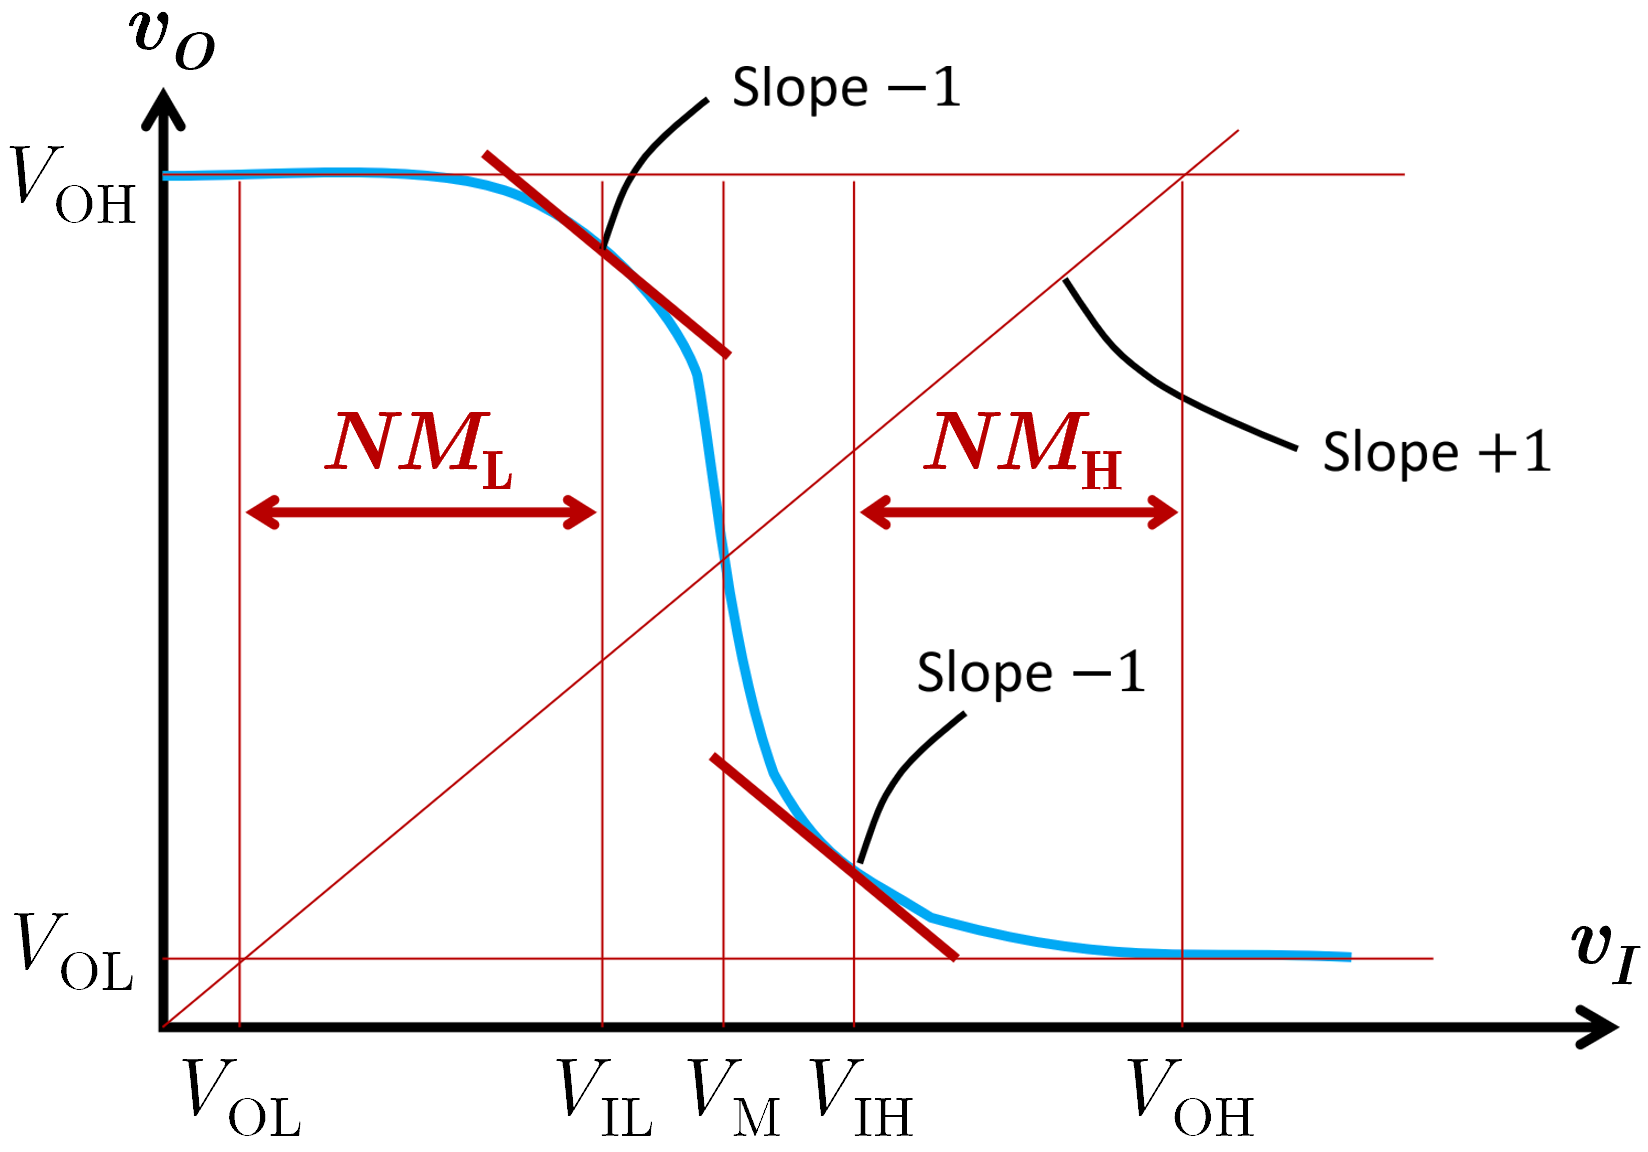
\includegraphics[width=6.33cm]{CMOS_vtf.png}}
	\caption{CMOS反相器}
	\vspace{-1em}
\end{figure}

在\(v_I=V_\mrm{IH}\)处,\(\begin{cases}
	v_{SG,P} \ge V_\mrm{th},\\ v_{DG,P} \le V_\mrm{th}, 
\end{cases}\)即\(Q_P\)工作在 Saturation区;\(\begin{cases}
	v_{GS,N} \ge V_\mrm{th},\\ v_{GD,N} \ge V_\mrm{th}, 
\end{cases}\)即\(Q_N\)工作在 Triode区。于是列式 
\begin{equation*}
	\begin{cases}
		i_{D,P}=i_{D,N}, \\
		i_{D,N}=\big(\mu_\textsl{n}C_{ox}\big)\left(\dfrac{W}{L}\right)_\textsl{n}\left[\big(v_{GS,N}-V_\mrm{th}\big)v_{DS,N}-\dfrac{1}{2}v_{DS,N}^{2}\right], \\[3pt]
		i_{D,P}=\dfrac{1}{2}\big(\mu_\textsl{p}C_{ox}\big)\left(\dfrac{W}{L}\right)_\textsl{p}\big(v_{SG,P}-V_\mrm{th}\big)^{2}, \\
		\dfrac{\dif v_O}{\dif v_I} = \dfrac{\dif v_{DS,N}}{\dif v_{GS,N}} = -1
	\end{cases}
	\quad\xLongrightarrow{\text{假设~}(\mu_\textsl{n}C_{ox})\left(\frac{W}{L}\right)_\textsl{n} = (\mu_\textsl{p}C_{ox})\left(\frac{W}{L}\right)_\textsl{p}}\quad
	V_\mrm{IH} = \dfrac{5V_{dd} - 2 V_\mrm{th}}{8}
\end{equation*}
同理即得\(V_\mrm{IL} = \dfrac{3V_{dd} + 2V_\mrm{th}}{8}\)。若进一步假设\(V_\mrm{OL} = 0\),\(V_\mrm{OH} = V_{dd}\),则可求得\(NM_\mrm{L} = NM_\mrm{H} = \dfrac{3V_{dd} + 2V_\mrm{th}}{8}\)。

下面向 CMOS反相器 输入 阶跃电压信号,考察其时间和能量的动态特性。

\paragraph{传播延迟}

对 CMOS反相器 输入 阶跃电压信号,其实际输出响应如图~\ref{Pic: CMOS Inverter delay}~所示,变化趋势类似电容的充放电过程,于是不妨将电路中所有容性成分集中为电容\(C\),而MOS管保持理想,如图~\ref{Pic: CMOS Inverter C}。定义输出电压从低电位到高电位、从高电位到低电位的过程中,越过最高电平一半所用的时间为\tboba{传输延时}~\(t_\mrm{PLH},t_\mrm{PHL}\)。

\begin{figure}[ht!]
	\centering
	\subfloat[阶跃响应]{\label{Pic: CMOS Inverter delay}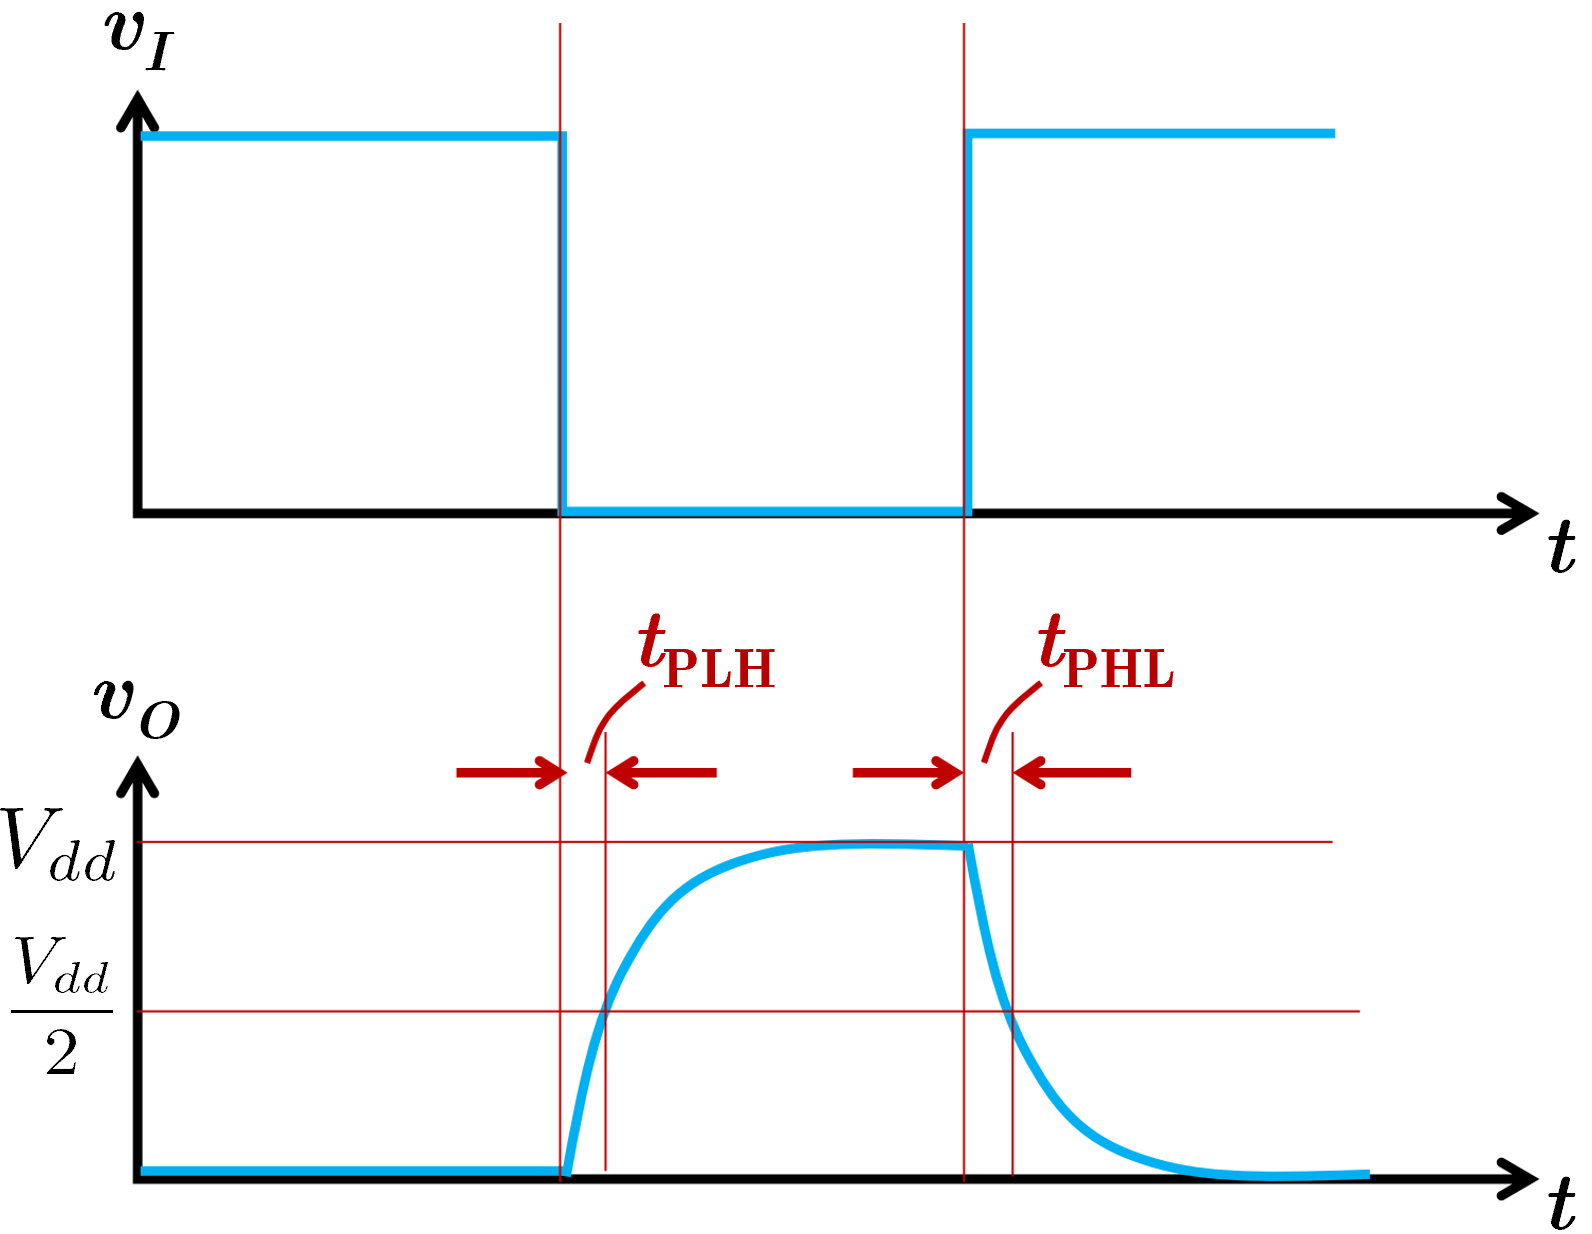
\includegraphics[width=6.33cm]{CMOS_Pd.png}}
	\quad
	\subfloat[等效电路]{\label{Pic: CMOS Inverter C}
		\begin{circuitikz}
			\draw (0,0) node[left]{\(v_I\)} to[short, o-] ++(0.8,0) coordinate(in)
				-- ++(0,0.8) -- ++(0.5,0) node[pmos, anchor=G](Pmos){\(Q_P\)}
			(Pmos.S) node[vcc]{\(V_{dd}\)}
			(in) -- ++(0,-0.8) -- ++(0.5,0) node[nmos, anchor=G](Nmos){\(Q_N\)}
			(Nmos.S) node[ground]{}
			(Nmos.D) -- (Pmos.D)
			(in -| Nmos.D) -- ++(0.8,0) coordinate(cap) to[short, -o] ++(0.8,0) node[right]{\(v_O\)}
			(cap) to[C, l=\(C\)] ++(0,-1) node[ground]{}
			;
		\end{circuitikz}
	}
	\caption{CMOS反相器的传播延迟}
	\vspace{-1em}
\end{figure}

下面考察输出由低电平到高电平的过程。
\begin{itemize}
	\item 输入在\(V_{dd}\),输出在GND时,\(Q_P\)在 Cutoff区,\(Q_N\)在 Triode区;
	\item 当输入跳变到GND后,\(Q_N\)进入 Cutoff区保持关断,\(Q_P\)进入 Saturation区,有\(i_D = \dfrac{1}{2}k_\textsl{p}(v_{SG,P}-V_\mrm{th})^2 = \dfrac{1}{2}k_\textsl{p}(V_{dd}-V_\mrm{th})^2 \)为恒值,直到\(v_{DG,P} = v_O\)达到\(V_\mrm{th}\)。于是 
	\[
		t_\mrm{PLH1} = \dfrac{C \Dif v_O }{i_D } = \dfrac{2CV_\mrm{th}}{k_\textsl{p}(V_{dd}-V_\mrm{th})^2}
	\]
	\item 当\(v_{DG,P} = v_O\)达到\(V_\mrm{th}\)后,\(Q_P\)进入 Triode区,有\(i_D = k_\textsl{p}\left[ (v_{SG,P}-V_\mrm{th})v_{SD,P} - \dfrac{1}{2}v_{SD,P}^2 \right] = k_\textsl{p}\Big[ (V_{dd}-V_\mrm{th})\cdot(V_{dd}-v_O) - \dfrac{1}{2}(V_{dd}-v_O)^2 \Big]\),于是
	\[
		t_\mrm{PLH2} = \int_{V_\mrm{th}}^\frac{V_{dd}}{2} \dfrac{C \dif v_O}{i_D}
		= \dfrac{C}{k_\textsl{p}} \int_{V_\mrm{th}}^\frac{V_{dd}}{2} \dfrac{ \dif v_O}{(V_{dd}-V_\mrm{th})(V_{dd}-v_O) - \dfrac{1}{2}(V_{dd}-v_O)^2}
		= \dfrac{C}{k_\textsl{p}(V_{dd}-V_\mrm{th})} \ln \dfrac{3V_{dd} - 4V_\mrm{th}}{V_{dd}}
	\]
\end{itemize}
故总的传输延迟为
\equ{
	t_\mrm{PLH} = \dfrac{2CV_\mrm{th}}{k_\textsl{p}(V_{dd}-V_\mrm{th})^2} + \dfrac{C}{k_\textsl{p}(V_{dd}-V_\mrm{th})} \ln \dfrac{3V_{dd} - 4V_\mrm{th}}{V_{dd}}
}

\paragraph{能量消耗}

电容\(C\)放电过程中,耗散能量即为慢点所储能量,为\(E_\mrm{dissipated1} = \dfrac{1}{2}CV_{dd}^2\);充电过程中,耗散能量为电源供能与电容储能之差,即\(E_\mrm{dissipated2} = V_{dd}\dint_{t_\mrm{PLH}} i_D \dif t - \dfrac{1}{2}CV_{dd}^2 = \dfrac{1}{2}CV_{dd}^2\)。故,每个周期能量消耗为\(CV_{dd}^2\),动态耗能功率即\(P_\mrm{dyn} = fCV_{dd}^2\)。

\subsubsection{CMOS逻辑门电路}

CMOS逻辑门电路是CMOS反相器的扩展或推广:逆变器由NMOS下拉晶体管和PMOS上拉晶体管组成,以输入电压与期望输出相反的方式工作。CMOS逻辑门将这两个晶体管扩展为如图~\ref{Pic: CMOS Gate Mode}~所示的两个网络:由NMOS晶体管构成的\tboba{下拉网络(PDN)}和由PMOS晶体管构成的\tboba{上拉网络(PUN)\hskip-0.5em}。

这两个网络由一组输入变量以互补的方式控制。在所有期望低输出(\(Y \eqcirc 0\)\footnote{在本文档中,为区分电压值和逻辑值两种情况,逻辑值的相等使用「\(\eqcirc\)」(\texttt{\backslash eqcirc})表示。})的输入组合下,PDN将导通,将输出节点接通到地,使得输出端\(v_Y = 0\),同时PUN关断,\(V_{dd}\)和地面之间不存在直流路径;在所有期望高输出(\(Y \eqcirc 1\))的输入组合下,PUN将导通,将输出节点拉到\(V_{dd}\),使得输出电压\(v_Y = V_{dd}\),同时PDN关断,电路中同样不存在\(V_{dd}\)和地之间的直流路径。

\begin{figure}[!ht]
	\centering
	\vspace{-0.5em}
	\begin{circuitikz}
		\draw [ fill={rgb,255:red,206; green,218; blue,238} ] (3.75,13) rectangle  node {\normalsize \shortstack{PDN\\(NMOS)}} (5.75,11.5);
		\draw [ fill={rgb,255:red,243; green,221; blue,227} ] (3.75,15.5) rectangle  node {\normalsize \shortstack{PUN\\(PMOS)}} (5.75,14);
		\draw [](4.75,14) to[short] (4.75,13);
		\draw [](4.75,13.5) to[short] (5.75,13.5);
		\draw [](4.75,15.5) to[short] (4.75,16) node[vcc]{$V_{dd}$};
		\draw [](4.75,11.5) to[short] (4.75,11) node[ground]{};
		\draw [](3.75,14.75) to[short, -o] (2.75,14.75) node[left] {$B$};
		\draw [](3.75,15.25) to[short, -o] (2.75,15.25) node[left] {$A$};
		\draw [](3.75,14.25) to[short, -o] (2.75,14.25) node[left] {$C$};
		\draw [](3.75,12.75) to[short, -o] (2.75,12.75) node[left] {$A$};
		\draw [](3.75,12.25) to[short, -o] (2.75,12.25) node[left] {$B$};
		\draw [](3.75,11.75) to[short, -o] (2.75,11.75) node[left] {$C$};
		\draw [](5.75,13.5) to[short, -o] (6.75,13.5) node[right] {$Y$};
	\end{circuitikz}
	\caption{CMOS逻辑门电路的一般模式}\label{Pic: CMOS Gate Mode}
	\vspace{-0.5em}
\end{figure}

\ctikzset{logic ports=ieee}

\bu[非门]{
	输入信号\(A\)做非运算输出\(Y\),记作\cbox{
		\draw (0,0) node[left]{\(A\)} to[short, o-] ++(0.5,0) node[not port, anchor=in](Not){}
		(Not.out) to[short, -o] ++(0.5,0) node[right]{\(Y\)};
	}。
}{
	\(Y \eqcirc \overline{A}\)。
}

前面的CMOS反相器输出与输入的关系为\begin{tabular}{c|c}
	\(v_I\) & \(v_O\) \\
	\hline
	\(V_{dd}\) & GND \\
	GND & \(V_{dd}\)
\end{tabular},这就是一个CMOS非门。

\bu[与非门]{
	输入信号\(A,B\)做与非运算输出\(Y\),记作\cbox{
		\draw (0,0) node[left]{\(A\)} to[short, o-] ++(0.5,0) node[nand port, anchor=in 1](Not){}
		(Not.in 2) to[short, -o] ++(-0.5,0) node[left]{\(B\)}
		(Not.out) to[short, -o] ++(0.5,0) node[right]{\(Y\)};
	}。
}{
	\(Y \eqcirc \overline{A \cdot B}\)。
}

如图~\ref{Pic: CMOS nand}~所示为一种CMOS与非门逻辑电路。当\(A\)或\(B \)有一个输入为 GND 时,对应的\(Q_{PA}\)和\(Q_{PB}\)总有至少一路导通到\(V_{dd}\),而接地路线上\(Q_{NA}\)和\(Q_{NB}\)总有至少一处断开,输出\(Y = V_{dd}\)。
\newcommand{\pmosin}[2]{% 1: input signal label; 2: D point
	\draw #2 -- ++(0,0.1) node[pmos, anchor=D](Pin#1){\(Q_{P#1}\)}
		(Pin#1.G) to[short, -o] ++(-0.2,0) node[left](Pin#1-G){\(#1\)}
		(Pin#1.S) -- ++(0,0.1) coordinate(Pin#1-S)
	;
}
\newcommand{\nmosin}[2]{% 1: input signal label; 2: D point
	\draw #2 -- ++(0,-0.1) node[nmos, anchor=D](Nin#1){\(Q_{N#1}\)}
		(Nin#1.G) to[short, -o] ++(-0.2,0) node[left](Nin#1-G){\(#1\)}
		(Nin#1.S) -- ++(0,-0.1) coordinate(Nin#1-S)
	;
}
\begin{figure}[!ht]
	\centering
	\vspace{-0.5em}
	\cbox{
		\draw (0,0) to[short, -o] ++(2.5,0) node[right]{\(Y\)};
		\pmosin{A}{(0,0)}
		\pmosin{B}{(2,0)}
		\nmosin{A}{(1,0)}
		\nmosin{B}{(NinA-S) ++(0,0.4)}
		\draw (PinA-S) node[vcc]{\(V_{dd}\)} (PinB-S) node[vcc]{\(V_{dd}\)} (NinB-S) node[ground]{};
	}
	\qquad
	\begin{tabular}{cc|c}
		\(A\) & \(B\) & \(Y\)\\
		\hline
		\(V_{dd}\) & \(V_{dd}\) & GND \\
		\(V_{dd}\) & GND & \(V_{dd}\) \\
		GND & \(V_{dd}\) & \(V_{dd}\) \\
		GND & GND & \(V_{dd}\)
	\end{tabular}
	\caption{一种CMOS与非门电路}\label{Pic: CMOS nand}
	\vspace{-0.5em}
\end{figure}

\bu[或非门]{
	输入信号\(A,B\)做或非运算输出\(Y\),记作\cbox{
		\draw (0,0) node[left]{\(A\)} to[short, o-] ++(0.5,0) node[nor port, anchor=in 1](Not){}
		(Not.in 2) to[short, -o] ++(-0.5,0) node[left]{\(B\)}
		(Not.out) to[short, -o] ++(0.5,0) node[right]{\(Y\)};
	}。
}{
	\(Y \eqcirc \overline{A + B}\)。
}
如图~\ref{Pic: CMOS nor}~所示为一种CMOS或非门逻辑电路。当\(A\)或\(B \)有一个输入为 \(V_{dd}\) 时,导通到\(V_{dd}\)路线上对应的\(Q_{PA}\)和\(Q_{PB}\)总有至少一处断开,而\(Q_{NA}\)和\(Q_{NB}\)总有至少一路接地,输出\(Y = \mrm{GND}\)。

\begin{figure}[!ht]
	\centering
	\vspace{-0.5em}
	\cbox{
		\draw (-1,0) to[short, -o] (1.5,0) node[right]{\(Y\)};
		\pmosin{B}{(0,0)}
		\pmosin{A}{(PinB-S) ++(0,-0.4)}
		\nmosin{A}{(-1,0)}
		\nmosin{B}{(1,0)}
		\draw (PinA-S) node[vcc]{\(V_{dd}\)} (NinA-S) node[ground]{} (NinB-S) node[ground]{};
	}
	\qquad
	\begin{tabular}{cc|c}
		\(A\) & \(B\) & \(Y\)\\
		\hline
		\(V_{dd}\) & \(V_{dd}\) & GND \\
		\(V_{dd}\) & GND & GND \\
		GND & \(V_{dd}\) & GND \\
		GND & GND & \(V_{dd}\)
	\end{tabular}
	\caption{一种CMOS或非门电路}\label{Pic: CMOS nor}
	\vspace{-0.5em}
\end{figure}

\zhu[逻辑门的扇入与伪NMOS逻辑电路]{
	扇入(Fan-in)表示单个逻辑门接受的最大输入信号数量。以上图~\ref{Pic: CMOS nand}~和图~\ref{Pic: CMOS nor}~中的逻辑门都只是 Fan-in 为2的情况,但这种构造每增加1个输入需要多出2个晶体管,不够节约硅片面积,也会引入更多寄生电容。图~\ref{Pic: p-NMOS}~是一种\tboqi{伪NMOS}~逻辑电路,通过调整\(Q_P\)和各\(Q_N\)的工艺参数,可以使得上下同时导通时\(Y \approx \mrm{GND}\),从而有\(Y \eqcirc \overline{A+B+C+D}\),而且每增加1个输入只需要多出1个晶体管。
	\begin{center}
		\cbox{
			\draw (0,0) to[short, -o] ++(6.5,0) node[right]{\(Y\)};
			\nmosin{A}{(0,0)}
			\nmosin{B}{(2,0)}
			\nmosin{C}{(4,0)}
			\nmosin{D}{(6,0)}
			\draw (3,0) -- ++(0,0.1) node[pmos, anchor=D](Pin){\(Q_P\)} 
				(Pin.G) -- ++(-0.2,0) node[ground]{}
				(Pin.S) -- ++(0,0.1) node[vcc]{\(V_{dd}\)}
				(NinA-S) node[ground]{}
				(NinB-S) node[ground]{}
				(NinC-S) node[ground]{}
				(NinD-S) node[ground]{}
			;
		}
	\end{center}
	\captionof{figure}{一种伪NMOS或非门}\label{Pic: p-NMOS}
}

\subsubsection{数字开关与动态逻辑电路}

单个的NMOS管可以用作开关,如图~\ref{Pic: single NMOS switch}~所示。

\begin{figure}[ht!]
	\vspace{-1.5em}
	\centering
	\subfloat[]{\begin{circuitikz}\label{Pic: single NMOS switch}
		\draw (5.5,11.5) to[Tnmos, name=N, invert, mirror] (7.5,11.5); 
		\draw (5.7,11.5) to[short, -o] (5.5,11.5) node[left] {$v_I$};
		\draw (7.3,11.5) to[short, -o] (7.5,11.5) node[right] {$v_O$};
		\draw (N.G) to[short, -o] (6.5,12.5) node[right] {$\phi$};
	\end{circuitikz}}\quad
	\subfloat[]{\begin{circuitikz}\label{Pic: single NMOS switch with cap}
		\draw (5.5,11.5) to[Tnmos, name=N, invert, mirror, l=\(Q_\mrm{s}\)] (7.5,11.5); 
		\draw (5.7,11.5) to[short, -o] (5.5,11.5) node[left] {$v_I$};
		\draw (7.3,11.5) to[short, -o] (8,11.5) node[right] {$v_O$};
		\draw (N.G) to[short, -o] (6.5,12.5) node[right] {$\phi$};
		\draw (7.5,11.5) to[C, l=\(C_L\)] (7.5,10.5) node[ground]{};
	\end{circuitikz}}\quad
	\subfloat[]{\begin{circuitikz}\label{Pic: single NMOS switch with inverter}
		\draw (5.5,11.5) to[Tnmos, name=N, invert, mirror, l=\(Q_\mrm{s}\)] (7.5,11.5); 
		\draw (5.7,11.5) to[short, -o] (5.5,11.5) node[left] {$v_I$};
		\draw (7.3,11.5) to[short, -o] (7.5,11.5) node[below]{$v_x$};
		\draw (N.G) to[short, -o] (6.5,12.5) node[right] {$\phi$};
		\draw (7.5,11.5) to[short, o-] ++(0.4,0) coordinate(in)
			-- ++(0,0.8) -- ++(0.5,0) node[pmos, anchor=G](Pmos){\(Q_P\)}
		(Pmos.S) node[vcc]{\(V_{dd}\)}
		(in) -- ++(0,-0.8) -- ++(0.5,0) node[nmos, anchor=G](Nmos){\(Q_N\)}
		(Nmos.S) node[ground]{}
		(Nmos.D) -- (Pmos.D)
		(in -| Nmos.D) -- ++(0.8,0) coordinate(cap) to[short, -o] ++(0.5,0) node[right]{\(v_O\)}
		(cap) to[C, l=\(C_L\)] ++(0,-1) node[ground]{}
		;
	\end{circuitikz}}
	\caption{单NMOS开关}
	\vspace{-1em}
\end{figure}

由于电路中各种寄生电容的存在,单NMOS开关输出端的阶跃响应也有传播延迟,可看作图~\ref{Pic: single NMOS switch with cap}~电路。但与前面反相器的响应不同的是,NMOS导通时要求\(v_{GS,N} = \phi - v_O > V_\mrm{th}\),即\(v_O < \phi - V_\mrm{th} \le V_{dd} - V_\mrm{th}\),则\(V_\mrm{OH} = V_{dd} - V_\mrm{th}\)比供电电压低。这导致\textbf{噪声门限减小},若以此控制一个CMOS反相器的输入信号(如图~\ref{Pic: single NMOS switch with inverter}),各MOS管相匹配,则\(v_{SG,P} = V_{dd} - v_x > |V_\mrm{th}|\),即\(Q_P\)将始终打开。类似地,若使用PMOS作开关,由于\(v_{SG,N} = v_O - \phi > V_\mrm{th}\)的限制,\(V_\mrm{OL} = V_\mrm{th}\)比GND高。

单NMOS、单PMOS开关分别有不能得到理想高电平、低电平的问题。若将其并联为图~\ref{Pic: CMOS tg}~电路,并令\(\phi = V_{dd}\),则\(v_I\)跳变到\(V_{dd}\)时,\(Q_N\)偏置到 Saturation区,负载电容充电至\(V_{dd} - V_\mrm{th}\),此时\(Q_N\)关断但\(Q_P \)仍导通,于是保证了\(V_\mrm{OH} = V_{dd}\);由MOS管源极和漏极的对称性,即也可保证\(V_\mrm{OL}=0\)。而当\(\phi=0\)时,\(Q_P\)、\(Q_N\)均只能在 Cutoff区,即切断了\(v_I\)与\(v_O\)的电路联系。

\begin{figure}[!ht]
	\centering
	\vspace{-0.5em}
	\cbox{
		\draw (0,0) node[left]{\(v_I\)} to[short, o-] ++(0.5,0) coordinate(in)
		(in) -- ++(0,0.5) to[Tpmos, name=P, invert, mirror] ++(2,0) -- ++(0,-0.5) coordinate(out) to[short, -o] ++(1,0) node[right]{\(v_O\)}
		(in) -- ++(0,-0.5) to[Tnmos, name=N, invert] ++(2,0) -- ++(0,0.5)
		++(0.5,0) to[C, l=\(C\)] ++(0,-1) node[ground]{}
		(P.G) to[short, -o] ++(0,0.2) node[above]{\(\bar{\phi}\)}
		(N.G) to[short, -o] ++(0,-0.2) node[below]{\(\phi\)}
		;
		\draw (1.5,0.5) node[below] {\(Q_P\)} (1.5,-0.5) node[above] {\(Q_N\)};
	}
	\caption{CMOS传输门}\label{Pic: CMOS tg}
	\vspace{-1em}
\end{figure}

\bu[传输门]{
	信号\(\phi\)控制\(X\)到\(Y\)的传输,记作
	\cbox{
		\draw (0,0) node[left]{\(X\)} to[short, o-] ++(0.2,0) node[ieee double tgate, anchor=in](TG){} 
		(TG.out) to[short, -o] ++(0.2,0) node[right]{\(Y\)}
		(TG.up) to[short, -o] ++(0,0.2) node[above]{\(\bar{\phi}\)}
		(TG.down) to[short, -o] ++(0,-0.2) node[below]{\(\phi\)}
		;
	}。
}{
	当\(\phi \eqcirc 1\)时,\(Y \eqcirc X\)。
}

CMOS传输门电路的缺点在于使用的晶体管数目较多,不利于节省硅片面积。如果在特定要求情境下,可以\textbf{将开关功能与逻辑运算功能结合}构造电路,则可以节省一些面积。
\newcommand{\pmosil}[3]{% 1: input signal text label; 2: input signal tex lavel; 3: D point
	\draw #3 -- ++(0,0.1) node[pmos, anchor=D](Pin#1){\(Q_{P#2}\)}
		(Pin#1.G) to[short, -o] ++(-0.2,0) node[left](Pin#1-G){\(#2\)}
		(Pin#1.S) -- ++(0,0.1) coordinate(Pin#1-S)
	;
}
\newcommand{\nmosil}[3]{% 1: input signal text label; 2: input signal tex lavel; 3: D point
	\draw #3 -- ++(0,-0.1) node[nmos, anchor=D](Nin#1){\(Q_{N#2}\)}
		(Nin#1.G) to[short, -o] ++(-0.2,0) node[left](Nin#1-G){\(#2\)}
		(Nin#1.S) -- ++(0,-0.1) coordinate(Nin#1-S)
	;
}
\begin{example}[3]
	讨论下面电路中,控制信号\(\phi\)不同时,输出信号\(Y \)与信号\(A,B\)的关系。
	\begin{center}
		\cbox{
			\draw (-1,0) to[short, -o] (1.5,0) node[right]{\(Y\)};
			\pmosil{phi}{\phi}{(0,0)}
			\nmosin{A}{(-1,0)}
			\nmosin{B}{(1,0)}
			\nmosil{phi}{\phi}{(NinA-S) ++(1,0)}
			\draw (NinA-S) -- (NinB-S) (Ninphi-S) node[ground]{} (Pinphi-S) node[vcc]{\(V_{dd}\)};
		}
	\end{center}
	\begin{solution}
		\(\phi \eqcirc 0\)时,\(Q_{P\phi}\)导通而\(Q_{N\phi}\)关断,\(Y \eqcirc 1\),与\(A,B\)无关;\(\phi \eqcirc 1\)时,\(Q_{P\phi}\)关断而\(Q_{N\phi}\)导通,\(Y\)接到地仅需\(A,B\)中有一个接到\(V_{dd}\),即\(Y \eqcirc \overline{A+B}\)。
	\end{solution}
\end{example}
综合来看,上例中实际上有\(Y \eqcirc \overline{A+B} + \overline{\phi} \eqcirc \overline{(A+B)\cdot\phi}\)。但其中,\(\phi \eqcirc 1\)时\(Y \eqcirc \overline{A+B}\)要求\(Q_{NA},Q_{NB}\)全部关断时\(Y \eqcirc 1\),因此必须保证在取\(\begin{cases}
	\phi \eqcirc 1,\\[-2pt] A \eqcirc 1, \\[-3pt] B \eqcirc 1
\end{cases}\)之前有\(Y \eqcirc 1\),即在这之前\(\phi \eqcirc 0\)。一般\(\phi\)设为时钟信号。

\subsubsection{反馈回路与存储电路}

前面所研究的逻辑电路被称为\tboba{组合电路},它们的输出只取决于输入的现值。因此,这些电路没有存储能力。存储电路是数字系统的重要组成部分,包含存储的逻辑电路称为\tboba{顺序电路};也就是说,它们的输出不仅取决于输入的现值,还取决于输入的先前值。

\begin{example}[3]
	用时钟信号\(\phi\)控制如图~\ref{Pic: D Flip Flop}~所示的电路,分析输出信号\(Q\)。\label{e.g: D Flip Flop}
	\begin{figure}[!ht]
		\centering
		\vspace{-1em}
		\subfloat[]{\label{Pic: D Flip Flop}\begin{circuitikz}
			\draw (0,0) node[left]{\(D\)} to[Tnmos, name=N, o-, invert, mirror] ++(1.5,0) node[above]{\(v_1\)}
				to[inline not=\(\hspace{-0.5em}I_1\)] ++(1.5,0) node[above]{\(v_2\)}
				to[inline not=\(\hspace{-0.5em}I_2\), color=meihong!75!black] ++(1.5,0) node[above](fst){\(v_3\)}
				to[short, -o] ++(0.5,0) node[right]{\(Q\)}
			(fst.south) -- ++(0,-1) to[Tnmos, name=Nf] ++(-3,0) -- ++(0,1);
			\draw (0.75,0) node[below] {\(Q_1\)} (3,-1) node[above] {\(Q_2\)};
			\draw (N.G) to[short, -o] ++(0,0.2) node[above]{\(\overline{\phi}\)} (Nf.G) to[short, -o] ++(0,-0.2) node[below]{\(\phi\)};
		\end{circuitikz}}
		\quad
		\subfloat[]{\label{Pic: Double inverter}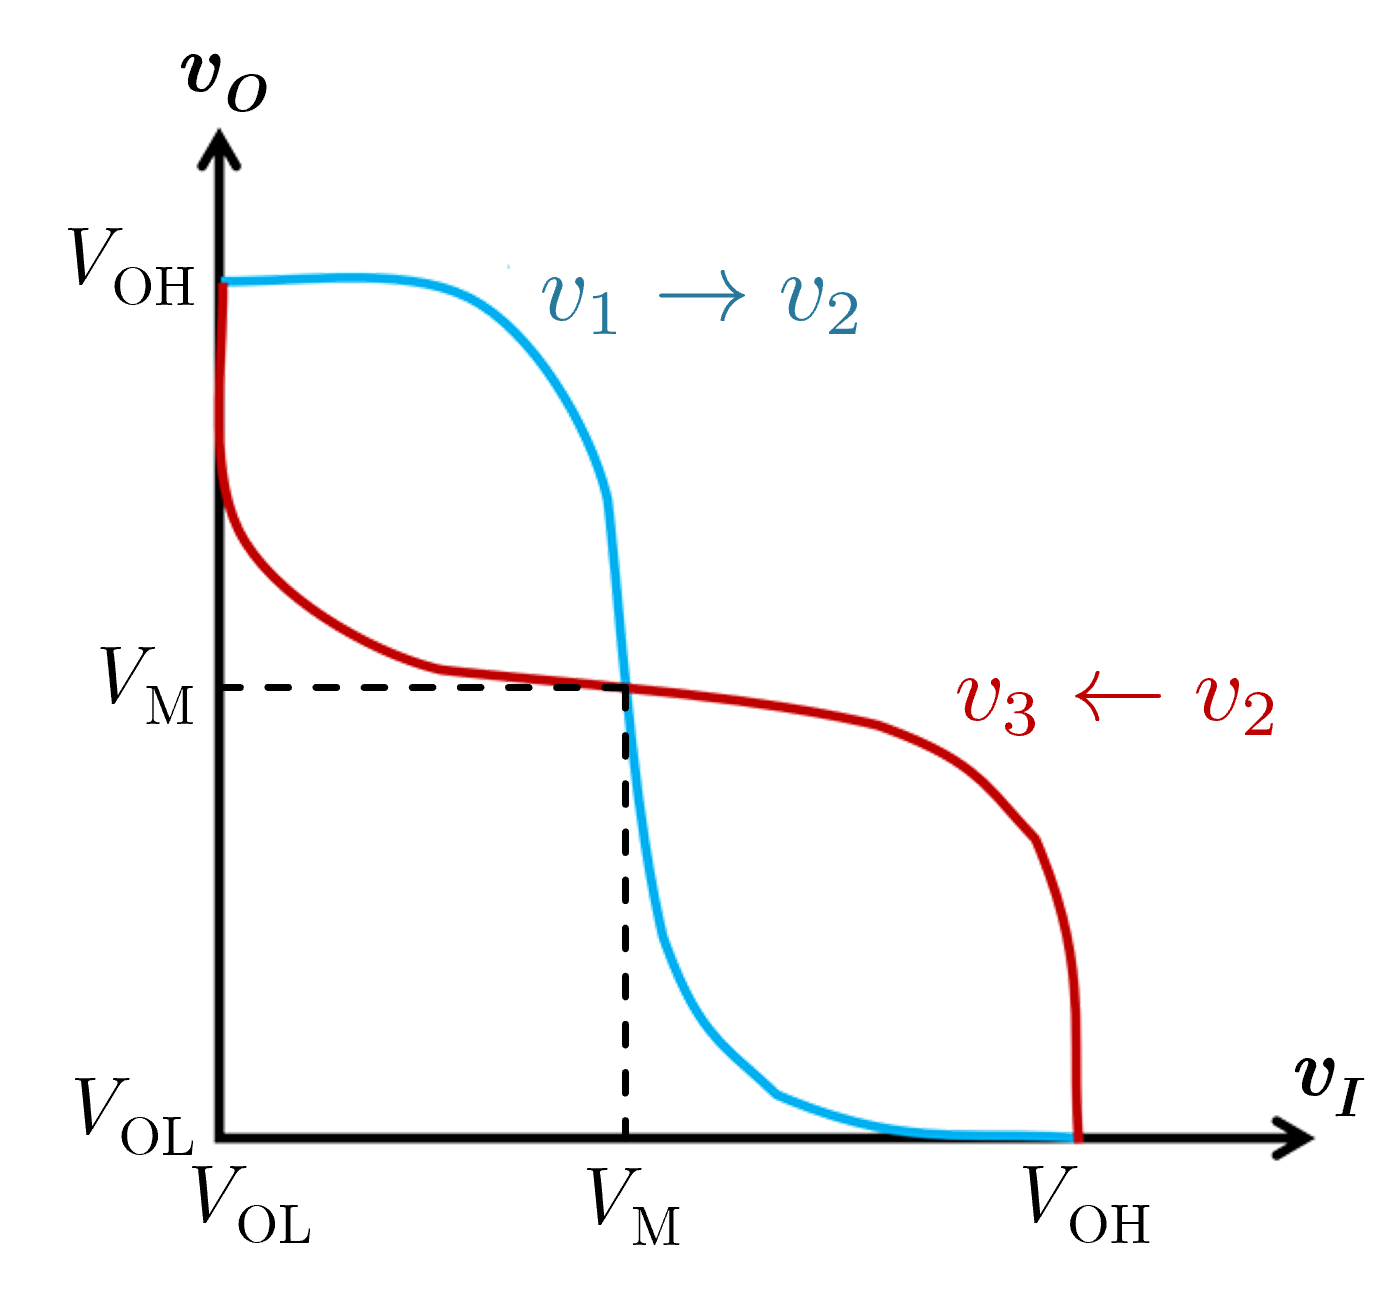
\includegraphics[width=5.04cm]{double inverter.png}}
		\caption{一个D触发器电路}
		\vspace{-1em}
	\end{figure}
\begin{solution}
	\(\phi \eqcirc 0\)时,\(Q_1\)打开、\(Q_2\)关闭,可直接充电至\(Q \eqcirc D\)。
	
	\(\phi \eqcirc 1\)时,\(Q_1\)关闭、\(Q_2\)打开,反馈回路将两个反相器的输出信号送回输入。据图~\ref{Pic: CMOS Inverter delay}~所示的传输曲线,得此时\(v_1,v_2,v_3\)的关系如图~\ref{Pic: Double inverter}。读图可知,\((V_\mrm{M},V_\mrm{M})\)不是一个稳定的平衡点,因此输出端\(v_3\)只可能取为\(V_\mrm{OH}\)或\(V_\mrm{OL}\),即\(Q\)保持前面输入的\(D\)不变。
\end{solution}
\end{example}

将例~\ref{e.g: D Flip Flop}~中的反相器用CMOS电路展开,调整两个NMOS开关的位置,就得到图~\ref{Pic: Memory cell}~所示的存储单元。

\begin{figure}[ht!]
	\centering
	\begin{circuitikz}
		\circuitikzset{bipoles/crossing/size=0.3,}
		\draw (6,14) node[vcc]{\(V_{dd}\)} to[Tpmos, name=M1] (6,12.5); 
		\draw (M1.G) to[short] (7,13.25);
		\draw (10-1,12.5) to[Tpmos, name=M2] (10-1,14) node[vcc]{\(V_{dd}\)}; 
		\draw (M2.G) to[short] (9-1,13.25);
		\draw (6,11.75) to[Tnmos, name=M3] (6,10.25); 
		\draw (M3.G) to[short] (7,11);
		\draw (10-1,10.25) to[Tnmos, name=M4] (10-1,11.75); 
		\draw (M4.G) to[short] (9-1,11);
		\draw (3.5,11.75) to[Tnmos, name=M5] (6,11.75); 
		\draw (4.75,12.75) to[short] (M5.G);
		\draw (10-1,12.5) to[Tnmos, name=M6] (12.5-1,12.5); 
		\draw (M6.G) to[short] (11.25-1,13.5);
		\draw [](6,12.5) to[short] (6,11.75);
		\draw [](10-1,12.5) to[short] (10-1,11.75);
		\draw [](7,13.25) to[short] (7.25,13.25);
		\draw [](7.25,13.25) to[short] (7.25,11);
		\draw[] (7.25,11) to[short] (7,11);
		\draw[] (9-1,13.25) to[short] (8.75-1,13.25);
		\draw [](8.75-1,13.25) to[short] (8.75-1,11);
		\draw [](8.75-1,11) to[short] (9-1,11);
		\draw [](6,11.75) -- (7,11.75) to[crossing, black] (8.5-1,11.75);
		\draw[] (10-1,12.5) -- (8,12.5) to[crossing, black] (7.5,12.5);
		\draw [](7.25,12.5) to[short] (7.5,12.5);
		\draw [](8.5-1,11.75) to[short] (8.75-1,11.75);
		\draw (6,10.25) node[ground]{};
		\draw (10-1,10.25) node[ground]{};
		\draw [](3.5,10.5-0.5) to[short] (3.5,16.5-1);
		\draw [](12.5-1,10.5-0.5) to[short] (12.5-1,16.5-1);
		\draw [](3,16-1) to[crossing, black] (4,16-1);
		\draw [](12-1,16-1) to[crossing, black] (13-1,16-1);
		\draw [](4,16-1) to[short] (12-1,16-1);
		\draw [](4.75,12.75) to[short] (4.75,16-1);
		\draw [](11.25-1,13.5) to[short] (11.25-1,16-1);
		\node [font=\small] at (13.25-1,16-1) {$WL$};
		\node [font=\small] at (2.75,16-1) {$WL$};
		\node [font=\small] at (3.5,10.25-0.5) {$\overline{BL}$};
		\node [font=\small] at (3.5,16.75-1) {$\overline{BL}$};
		\node [font=\small] at (12.5-1,16.75-1) {$BL$};
		\node [font=\small] at (12.5-1,10.25-0.5) {$BL$};
		\node at (6,11.75) [circ] {} ;
		\node at (6,11.75) [below left] {\(\overline{Q}\)} ;
		\node at (10-1,12.5) [circ] {};
		\node at (10-1,12.5) [below right] {\(Q\)};
	\end{circuitikz}
	\caption{一种随机存取存储器单元}\label{Pic: Memory cell}
\end{figure}

首先考虑读取操作,并假设该单元格正在存储一个1。在这种情况下,\(Q\)在高电平\(V_{dd}\),\(\overline{Q}\)在低电平GND。在读取操作开始之前,\(BL\)和\(\overline{BL}\)线路都被拉高到高电平范围,这个过程称为\textbf{预充电}。为了简化问题,这里假设\(BL\)和\(\overline{BL}\)的预充电电压为\(V_{dd}\),当字线被选择和接入晶体管被打开时,对电路的检查显示,唯一将导电的部分如图15

\subsection{振荡电路}

\subsubsection{负阻值与振荡器}

前面第~~节已经研究,RLC电路的振荡是一个能量衰减的过程。如果在电路中引入\tboba{负电阻},则电路信号的振荡有可能不再衰减。\textbf{负电阻是能量输入的一种体现。}

\begin{example}
	计算下面电路的小信号输入阻抗。
	\begin{center}
		\cbox{
			\draw (7.25,7.5) to[short, -o] (6.75,7.5) coordinate(in1);
			\draw (7.25,6.5) to[short, -o] (6.75,6.5) ;
			\draw (7.25,7.5) to[short] (10,7.5);
			\draw (7.25,6.5) to[short] (7.75,6.5);
			\draw (7.75,6.5) to[R, european, l=\(Z_1\)] (7.75,5.5);
			\draw (7.75,5.5) coordinate(gnd) to (7.75,5.25) node[ground]{};
			\draw (7.75,5.5) to[short] (10,5.5);
			\draw (10,7.5) to[R, european, l=\(Z_2\)] (10,5.5);
			\draw (7.75,6.5) to[short] (8.25,6.5) node[nmos, anchor=G](1){}
			(1.S) -- (gnd -| 1.S) (1.D) -- (in1 -| 1.D);
			\draw [ color={rgb,255:red,190; green,0; blue,0}, line width=0.5pt, short] (7,5.5) node[left]{\(\symbf{Z_\mrm{in}}\)} ++(0,-0.2) -- (7,8);
			\draw [ color={rgb,255:red,190; green,0; blue,0}, line width=0.5pt, -latex] (7,8) -- (7.5,8);
		}
	\end{center}
	\begin{solution}
		
	\end{solution}
\end{example}


\cbox{
	\draw (6,6.5) to (6,6.25) node[ground]{};
	\draw (6,6.5) to[short] (6,8.5);
	\draw (6,8.5) to[short, -o] (6.5,8.5) ;
	\draw (7.5,7.5) to[short, -o] (6.5,7.5) to[open, o-o, v<=\(v_{gs}\)] (6.5,8.5);
	\draw (7.5,7.5) to[R,l={ \small $R_S$}] (7.5,6.5);
	\draw (8.75,7.5) to[C,l={ \small $C_2$}] (8.75,6.5);
	\draw (8.75,7.5) to[C,l_={ \small $C_1$}] (8.75,8.5);
	\draw (7.5,8.5) to[short] (10,8.5);
	\draw (10,8.5) to[R,l={ \small $R_L$}] (10,7.5);
	\draw (7.5,8.5) to[american controlled current source,l={ \small $g_mv_{gs}$}] (7.5,7.5);
	\draw (7.5,8.5) to[L,l={ \small $L_1$} ] (7.5,9.5);
	\draw (10,7.5) to (10,7.25) node[ground]{};
	\draw (7.5,9.5) to (7.75,9.5) node[ground]{};
	\draw (10,8.5) to[short, -o] (10.5,8.5) node[right] {$v_\mrm{out}$};
	\draw (7.5,6.5) to (7.5,6.25) node[ground]{};
	\draw (8.75,6.5) to (8.75,6.25) node[ground]{};
}


\newpage
x
$\symbfup{XtRee}$
%----------------------------------------------------------
\end{document}

\subsubsection{Fourier变换与信号频谱}
对信号做~\tboba{Fourier变换},即将其分解为各种频率、强度的正弦波信号的和。
\begin{example}
	周期为$T$,峰值为$V$的对称方波电压信号
	$$v(t)=\left\{ \begin{NiceArray}{ll} V, & t\in \left[\dfrac{2kT}{2}\right.,\left.\dfrac{(2k+1)T}{2}\right), \\ -V, & t\in \left[\dfrac{(2k+1)T}{2}\right.,\left.\dfrac{(2k+2)T}{2}\right), \end{NiceArray} \right.k \in \mathbb{Z}$$
	可以转换为$v(t)=\dfrac{4V}{\pi}\sum\limits_{k=1}^\infty \dfrac{\sin (2k+1)\omega_0t}{2k+1}$,其中$\omega_0=\dfrac{2\pi}{T}$称为方波的\textbf{基频}。%\trans[基频]{fundamental frequency}
\end{example}
\de[频谱(frequency spectrum)]{
	给定信号$v(t)$,其 Fourier变换 的结果为$v(t)=\sum\limits_{k=1}^n V_k\sin \omega_kt$,将分解出的每个正弦波的$V_k$和$\omega_k$在直角坐标系$V-\omega$中成对描点,得到的曲线$V(\omega)$称为信号的\tboba{频谱}。
}
信号既可以由其时间波形表示,也可以由其频谱表示,分别称为\tboba{时域表示}%\trans[时域表示]{time-domain representation}
和\tboba{频域表示}%\trans[频域表示]{frequency-domain representation}
。信号$a$时域表示$v_a(t)$的频域表示形式常记作$V_a(\omega)$。

\subsubsection{信号数字化}

\subsubsection{信号放大的元件}
\bu[放大器(amplifier)]{
	不失一般性,\tboba{放大器}可以自左而右从入到出地记为
	\ctikzset{amplifiers/fill=bali!25!white}
	$\vcenter{\hbox{\begin{circuitikz}
		\draw (0,0) to[short, o-] ++(0.5,0) node[fd op amp, anchor=-](AMP){}; 
		\draw (AMP.+) to[short, -o] ++(-0.5,0) to[open, o-o] (0,0);
		\draw (AMP.out -) to[short, -o] ++(0.5,0) coordinate(TEMP);
		\draw (AMP.out +) to[short, -o] ++(0.5,0) to[open, o-o] (TEMP);
	\end{circuitikz}}}$(\texttt{fd op amp})。
	更常用的记法是
	$\vcenter{\hbox{\begin{circuitikz}
		\draw (0,0) coordinate(IN) to[short, o-, f^>=$i_I$] ++(1,0) node[plain mono amp, anchor=bin](AMP){}
		(AMP.down) -- ++(0,-0.5) node[ground](G){}
		(AMP.out) to[short, -o] ++(0.5,0) coordinate(OUT) to[short, o-, f_<=$i_O$] (AMP.bout)
		(G) to[short, *-o] (G -| IN)
		(G) to[short, *-o] (G -| OUT)
		;
	\end{circuitikz}}}$(\texttt{plain mono amp}),其中输入、输出侧存在公用端子,且同时接地,称为\tboba{电路地}。这个公用端子也可只画在输入侧。
}{
	将输入信号\textbf{线性}放大输出,放大效果由\tboba{放大器增益}~$A$刻画。
}
%\tranS[-6.5]{电路地}{circuit ground}\tranS[-4]{线性性}{linearity}
%\vspace{-\baselineskip}
\de[放大器增益(amplifier gain)]{
	\begin{wrapfigure}{r}{15em}
		\begin{circuitikz}
			\draw (0,0) coordinate(IN) to[short, o-, f^>=$i_I$] ++(1,0) node[plain amp, anchor=in up](AMP){}
			(AMP.in down) -- ++(0,-0.75) node[ground](G){}
			(AMP.out) to[short, -o] ++(0.5,0) coordinate(OUT) to[short, o-, f_<=$i_O$] (AMP.out)
			(G) to[short, *-o] (G -| IN)
			(IN) to[vsource, o-o, v_=$v_I$] (G -| IN) 
			(G) to[short, *-o] (G -| OUT)
			(OUT) to[open, o-o, v=$v_O$] (G -| OUT)
			;
		\end{circuitikz}
	\end{wrapfigure}
	在右边电路中,定义:
	\lineskip=4pt
	\lineskiplimit=2pt

	放大器的\tboba{电压增益}为放大器输出信号电压与输入信号电压的比值,记作$A_v$,即$A_v=\dfrac{v_O}{v_I}$;

	放大器的\tboba{电流增益}为放大器输出信号电流与输入信号电流的比值,记作$A_i$,即$A_i=\dfrac{i_O}{i_I}$;

	放大器的\tboba{功率增益}为放大器输出功率与输入功率的比值,记作$A_{p}$,即$A_{p}=\dfrac{p_O}{p_I}=A_vA_i$。
}
\zhu[放大器增益的单位]{
	\abovedisplayskip=2pt
	\belowdisplayskip=2pt
	放大器增益是个无量纲物理量,可以不标单位。为了体现电压增益、电流增益、功率增益之间的区分,也可以记上单位V/V、A/A、W/W;此时,可将数量级放入这些单位中,如MV/V、kA/A等。

	由于其无量纲的特性,放大器增益也可表示成对数形式,即\textbf{以分贝表示的增益},此时带单位dB以作区分。规定:
	\begin{align*}
		&\text{电压增益为}~A_v \ \symup{V/V} \Lr \text{电压增益为}~20\log_{10}|A_v| \ \symup{dB}\\[-5pt]
		&\text{电流增益为}~A_i \ \symup{A/A} \Lr \text{电流增益为}~20\log_{10}|A_i| \ \symup{dB}\\[-5pt]
		&\text{功率增益为}~A_p \ \symup{W/W} \Lr \text{功率增益为}~10\log_{10}A_p \ \symup{dB}
	\end{align*}
}

\subsubsection{放大器的电源}
放大器需要直流电源供电,提供增益的功率和电路内损失的功率。如图~\ref{Pic: 直流电源向放大器供电}~所示,电源内部有一点接地,将电源分为两部分,其中负极接地的称为\textbf{正电源},其正极接到放大器的$\mathtt{V^+}$端子;正极接地的称为\textbf{负电源},其负极接到放大器的$\mathtt{V^-}$端子。电路可以简化为图~\ref{Pic: 直流电源向放大器供电-简化形式}~形式。
\begin{figure}[ht!]
	\vspace{-1.5em}
	\centering
	\subfloat[直流电源向放大器供电]{
		\label{Pic: 直流电源向放大器供电}\begin{circuitikz}
			\draw (0,0) coordinate(IN) to[short, o-, f^>=$i_I$] ++(1,0) node[plain amp, anchor=in up](AMP){}
			(AMP.in down) -- ++(0,-0.75) node[ground](G){}
			(AMP.out) to[short, -o] ++(0.5,0) coordinate(OUT) to[short, o-, f_<=$i_O$] (AMP.out)
			(G) to[short, *-o] (G -| IN)
			(IN) to[vsource, o-o, v_=$v_I$] (G -| IN);
			\node at (G -| AMP.down)[jump crossing](C){};
			\draw (G) to[short, *-] (C.west) 
			(C.east) to[short, -o] (G -| OUT)
			(OUT) to[open, o-o, v=$v_O$] (G -| OUT)
			(AMP.up) to[short, -o] ++(0,0.4) node[right]{$\mathtt{V^+}$} to[short, o-] ++(0,0.5) -- ++(2.75,0) coordinate(U) -- ++(0,-2) to[battery1, -*, l=$V_{1}$] (G -| U) to[battery1, *-, l=$V_{2}$] ++(0,-0.6)
			(AMP.down) to[short, -o] ++(0,-0.4) node[right]{$\mathtt{V^-}$} to[short, o-] (G -| AMP.down) -- ++(0,-0.6) -- ++(2.75,0) to[open, f^<=$I_2$] ++(-1,0)
			(G -| U) to[short, *-o] (G -| OUT)
			(U) to[open, f_=$I_1$] ++(-1,0)
			;
		\end{circuitikz}
	}\qquad
	\subfloat[简化形式]{
		\label{Pic: 直流电源向放大器供电-简化形式}\begin{circuitikz}
			\draw (0,0) coordinate(IN) to[short, o-, f^>=$i_I$] ++(1,0) node[plain amp, anchor=in up](AMP){}
			(AMP.in down) -- ++(0,-0.75) node[ground](G){}
			(AMP.out) to[short, -o] ++(0.5,0) coordinate(OUT) to[short, o-, f_<=$i_O$] (AMP.out)
			(IN) to[vsource, o-, v_=$v_I$] (G -| IN) node[ground]{}
			(OUT) to[open, o-, v=$v_O$] (G -| OUT) node[ground]{}
			(AMP.up) to[short, -o] ++(0,0.4) node[right]{$\mathtt{V^+}$} to[short, o-] ++(0,0.5) node[vcc]{$V_{1}$} -- ++(0,0.3) to[open, f_=$I_1$] ++(0,-0.5)
			(AMP.down) to[short, -o] ++(0,-0.4) node[right]{$\mathtt{V^-}$} to[short, o-] ++(0,-0.5) node[vee]{$-V_{2}$} -- ++(0,-0.3) to[open, f^<=$I_2$] ++(0,0.5)
			;
		\end{circuitikz}		
	}
	\caption{带有直流电源的放大器电路图}\label{Pic: 带有直流电源的放大器电路图}
\end{figure}

图~\ref{Pic: 带有直流电源的放大器电路图}~电路中,电源对放大器的输入功率为$P_{\symup{dc}}=V_1I_1+V_2I_2$。若记放大器内部功率损耗为$P_{\symup{dissipated}}$,则由能量守恒有$$P_{\symup{dc}}+P_I=P_O+P_{\symup{dissipated}}$$

\begin{definition}
	\textbf{放大器的效率}\quad $\eta =\dfrac{P_O}{P_{\symup{dc}}}$。
\end{definition}

\subsubsection{放大器饱和}
放大器的输出电压有正负极限$L_+$、$L_-$,则其输入信号电压要在$\left(\dfrac{L_-}{A_v},\dfrac{L_+}{A_v}\right)$中才能保证线性放大。

\subsection{运算放大器}

\subsubsection{运算放大器及其模型}

\subsubsection{运算放大器基本电路}

\begin{example}
	在电路中考虑$\dfrac{v_o }{v_S }$的值:
	\begin{center}
		\cbox{
			\draw (0,0) coordinate(0) to[V, v=$v_S$, invert] ++(0,1.5) 
			to[R, l=$R_1$, -*] ++(1.5,0) coordinate(b) 
			-- ++(0.2,0) node[op amp, anchor=-](A){$A$}
			(A.+) -- ++(-0.2,0) coordinate(a) to[short, -*] (0 -| a)
			(b) -- ++(0,1) coordinate(b1) to[R, l=$R_2$] (b1 -| A.out)
			-- ++(0.2,0) coordinate(d1) to[short, -*] (A.out -| d1)
			(A.out) to[short, -o] ++(1.5,0) coordinate(v1)
			to[open, v=$v_o$, -o] (0 -| v1) to[short, o-] (0)
			(A.down) -- ++(0.5,0) coordinate(c) to[short, -*] (0 -| c) node[ground]{}
			;
		}
	\end{center}
\end{example}
\begin{solution}
	代入电路如下:
	\begin{center}
		\vspace{-1em}
		\cbox{
			\draw (0,0) coordinate(0) to[V, v=$v_S$, invert] ++(0,1.5) 
			to[R, l=$R_1$, -*] ++(1.5,0) coordinate(b) 
			to[R, l_=$R_i$, v^<, name=V1, voltage=european, voltage shift=1.5, *-*] (0 -| b)
			(b) -- ++(0,0.5) coordinate(b1) 
			to[R, l=$R_2$] ++(3.2,0) coordinate(d1) 
			to[short, -*] ++(0,-0.5) coordinate(d)
			to[short, *-o] ++(0.5,0) coordinate(v1)
			to[open, v=$v_o$, -o] (0 -| v1) to[short, o-] (0)
			(d) to[R, l=$R_o$, label distance=-7pt] ++(-1.5,0) coordinate(c) to[cV, v_=$Av_e$, -*, voltage shift=-0.7] (0 -| c) node[ground]{}
			;
			\draw[thin, -latex, ] 
			(V1-Vfrom) ++(0,-0.2) coordinate(St)
			(V1-Vto) ++(0,0.2) coordinate(En)
			(St) .. controls (V1-Vcont1) and (V1-Vcont2).. (En) node[pos=0.5, fill=black!5!white]{$v_e$};
		}
	\end{center}
\end{solution}